\documentclass[sigconf]{acmart}

\def\BibTeX{{\rm B\kern-.05em{\sc i\kern-.025em b}\kern-.08emT\kern-.1667em\lower.7ex\hbox{E}\kern-.125emX}}
\usepackage{libertine}
\usepackage{subfigure}
\usepackage{algorithm}
%\usepackage{algorithmic}
\usepackage{algpseudocode}
\usepackage{amsmath}
\usepackage{graphics}
\usepackage{epsfig}
\usepackage{multirow}
\usepackage{graphicx}
\usepackage{subfigure}
\usepackage{array}
\usepackage{fancyhdr}



\begin{document}

\title{Approximate Code: A Cost-Effective Erasure Coding Framework for Tiered Video Storage in Cloud Systems}

\author{Huayi Jin$^1$,
        Chentao Wu$^{1*}$,
        Xin Xie$^1$,
        Jie Li$^1$,
        Minyi Guo$^1$,
        Hao Lin$^2$,
        and Jianfeng Zhang$^2$}
\affiliation{%
    \institution{$^1$MoE Key Lab of Artificial Intelligence, AI Institute \& Department of Computer Science and Engineering, \\Shanghai Jiao Tong University, China}
    \institution{$^2$The Alibaba Group, China}
    \institution{$^*$Corresponding  author: wuct@cs.sjtu.edu.cn}
}

\renewcommand{\shortauthors}{Huayi Jin and Chentao Wu, et al.}

\begin{abstract}
Nowadays massive video data are stored in cloud storage systems, which are generated by various applications such as autonomous driving, news media, security monitoring, etc. Meanwhile, erasure coding is a popular technique in cloud storage to provide both high reliability and low monetary cost, where triple disk failure tolerant arrays (3DFTs) is a typical choice. Therefore, how to minimize the storage cost of video data in 3DFTs is a challenge for cloud storage systems. Although there are several solutions like approximate storage technique, they cannot guarantee low storage cost and high data reliability concurrently.

To address this challenge, in this paper, we propose Approximate Code, which is an erasure coding framework for tiered video storage in cloud systems. The key idea of Approximate Code is distinguishing the important and unimportant data with different capabilities of fault tolerance. On one hand, for important data, Approximate Code provides triple parities to ensure high reliability. On the other hand, single/double parities are applied for unimportant data, which can save the storage cost and accelerate the recovery process. To demonstrate the effectiveness of Approximate Code, we conduct several experiments in Hadoop systems. The results show that, compared to traditional 3DFTs using various erasure codes such as RS, LRC, STAR and TIP-Code, Approximate Code reduces the number of parities by up to $55\%$, saves the storage cost by up to $20.8\%$ and increase the recovery speed by up to $4.7$X when double nodes fail.
\end{abstract}

\ccsdesc[500]{Information systems~Distributed storage}
\ccsdesc[500]{Computer systems organization~Dependable and fault-tolerant systems and networks}


\copyrightyear{2019} 
\acmYear{2019} 
\setcopyright{acmcopyright}
\acmConference[ICPP 2019]{48th International Conference on Parallel Processing}{August 5--8, 2019}{Kyoto, Japan}
\acmBooktitle{48th International Conference on Parallel Processing (ICPP 2019), August 5--8, 2019, Kyoto, Japan}
\acmPrice{15.00}
\acmDOI{10.1145/3337821.3337869}
\acmISBN{978-1-4503-6295-5/19/08}

\keywords{Erasure Codes, Approximate Storage, Multimedia, Cloud Storage}
\maketitle


\section{Introduction}
For typical cloud storage systems such as Windows Azure \cite{calder2011windows} and Amazon AWS \cite{bermudez2013exploring}, erasure coding is a popular technique to provide both high reliability and low monetary cost \cite{EVENODD, RDP, BlaumRoth, XCode, CRS, TripleStar, TPtech, RSL}, where triple disk failure fault tolerant arrays (3DFTs) are widely used. Typical erasure codes can be divided into two categories, RS-based Codes \cite{RS} \cite{LRC} and XOR-based codes \cite{EVENODD, hcode, STAR, TIP}. RS-based codes are encoded based on the Galois Field(GF) computations \cite{RS}, which allow flexible configurations. XOR-based codes simplify the computations compared to RS-based code, but they suffer other issues like scalability \cite{wu2012sdm, jiang2016bdr}.

With the increasing demand on higher resolution and frame rate for video applications such as autonomous driving, news media, security monitoring, etc., massive storage devices are highly desired in cloud storage systems, which makes data centers much bigger.
Therefore, in this paper, we set out to answer the following question:

\textbf{In a cloud storage system, how to efficiently store tremendous video data in 3DFTs?}

To reduce the storage cost in cloud storage systems, a feasible solution is approximate storage. Approximate storage exposes unimportant data to errors, saving the overhead of redundant backups \cite{niklaus2018context, sampson2014approximate} , thus the data reliability cannot be guaranteed.
The second solution is using disk arrays like RAID-5\cite{menon1995performance} or RAID-6 \cite{RAID}, but the capability of fault tolerance is sacrificed.
Data compression\footnote{Typically, video coding (e.g., H.264 \cite{wiegand2003overview}) is a special type of data compression.}
is the third strategy to reduce the storage overhead \cite{ziv1977universal, ziv1978compression, deutsch1996deflate}, which needs to be collaborated with erasure codes for high reliability. However, the compression/decompression processes result in a large amount of computational overhead, which limits their usage in cloud systems. 
Therefore, existing solutions are difficult to provide low storage cost and high reliability simultaneously.

To address the challenge, in this paper, we propose Approximate Code, which is an erasure coding framework to provide a comprehensive solution for tiered video data storage in cloud systems. The key idea of Approximate Code is treating the important/unimportant data in different ways. For important data, we add additional parities to provide high capability of fault tolerance. On the other hand, the unimportant data are encoded with a minimum number of parities, which only supply the basic requirement of the recovery. When triple disks fail, the lost unimportant data can be reconstructed via a fuzzy manner.

We have the following contributions of this work,
\begin{enumerate}
\item We propose Approximate Code, which is a cost-effective framework to store video data in cloud storage systems.
\item Approximate Code can be implemented by combining various erasure codes in 3DFTs, such as RS, LRC, STAR Code, TIP-Code, etc.
\item We conduct several quantitative analysis and experiments according to different layouts of various erasure codes, and the results show that Approximate Code achieves a small number of parities, low storage cost, high single write performance, and fast data recovery under various failure scenarios.
\end{enumerate}

The rest of the paper is organized as follows. In Section \ref{RelatedWork}, we introduce related work and our motivation.
In Section \ref{ApCode}, the design of Approximate Code Framework will be illustrated in detail.
The evaluation is presented in Section \ref{evaluation} and the conclusion of our work is in Section \ref{Conclusion}.

\section{Related Work and Our Motivation}\label{RelatedWork}
In this section, we introduce the background of video storage, existing solutions to reduce storage cost and the motivation of this paper.
To facilitate the discussion, we summarize the symbols used in this paper in Table \ref{parameter}.

\begin{table}[]\footnotesize
\caption{The symbols used in this paper.}\label{parameter}
\centering
\begin{tabular}{|p{0.8cm}<{\centering}|p{6.4cm}|}
\hline
Symbols & \multicolumn{1}{c|}{Description} \\ \hline \hline
$k$ & the number of data nodes (in a local stripe) \\ \hline
$r$ & the number of parity nodes (in a local stripe) \\ \hline
$n$ & the number of all data and parity nodes in a local stripe. $n=k+r$ \\ \hline
$h$ & the number of local stripes to construct a global stripe \\ \hline
$g$ & the number of global parity nodes \\ \hline
$f$ & the number of failed nodes \\ \hline
$p$ & a prime number \\ \hline
$N$ & total number of all nodes ($N=h*(k+r)+g$) \\ \hline
$C_{i,j}$ & the element at the $i$-th row and $j$-th column \\ \hline
$A_{i,j}$ &  the coefficient of $C_{ij}$ in the Galois Field \\ \hline
$D_i$ & a data node \\ \hline
$P_{I}$ & the mathematical expectation of important data being recoverable under faults that exceed fault tolerance \\ \hline
$P_{U}$ & the mathematical expectation of unimportant data being recoverable under faults that exceed fault tolerance \\ \hline
$\oplus$ & an XOR operation \\ \hline
$\binom{n}{k}$ & the number of $k$-combinations from $n$ elements\\ \hline
LP & the local parity node \\ \hline
GP & the global parity node \\ \hline
ID & the important data in a video file \\ \hline
UD & the unimportant data in a video file \\ \hline
\end{tabular}

\end{table}


\subsection{Basis of Video Storage}\label{video storage}
For normal high-definition (HD, resolution 1280$\times$720, 8-bit, 30 fps) video, the amount of raw video data in 1 minute is 4.63 GB, so video data is usually encoded by lossy compression algorithms before storage.

\subsubsection{Video coding}
H.264 \cite{wiegand2003overview} is one of the advanced algorithms. This coding technique is widely used on platforms such as YouTube because it has higher compression ratio and lower complexity than its predecessors. For a normal HD video file as mentioned above, H.264 can reduce its size by about 10 times, only 443.27MB.

H.264 classifies all frames into three different categories,
\begin{enumerate}
    \item I frame: A frame that is self-contained, which means it can be decoded independently.
    \item P frame: A frame holds the changes compared to the previous frame, which saves the storage space by leaving out redundant information.
    \item B frame: A frame decreases the storage space as well by utilizing the data of both the preceding and following frames.
\end{enumerate}
A group of pictures (GOP) consists of one I frame followed by a number of consecutive P and B frames, as shown in Figure \ref{H264-IPB}.
Within each GOP, the I frame is the most significant because all other frames rely on it for recovery. P frames are the second important, and B frames have the least value.
Based on this feature, a special program can be designed to get the important video frames.

\begin{figure}[ht]
\centering
\includegraphics[width=0.35\textwidth]{photo/H264_IPB.pdf}
\caption{A sample of GOPs in H.264.}
\label{H264-IPB}
\end{figure}


\subsubsection{Video Frame Recovery}
In the circumstance of video approximate storage, it's common to lose some frames and make the video incompleted. However, the lost frames can still be recoverable with the benefit of powerful deep learning techniques. One of them is named video frame interpolation \cite{meyer2015phase, niklaus2018context, van2017frame}.

%Video frame interpolation is one of the basic video processing techniques, an attempt to synthetically produce one or more intermediate video frames from existing ones. This is a technique that can model natural motion within a video, and generate frames according to the model.

\subsection{Existing Erasure Codes}\label{existEC}
Reliability is a critical issue since disk failures are typical in storage systems. To improve the reliability of storage systems, several RAID forms (e.g., RAID-5, RAID-6, 3DFTs) and erasure codes are proposed by researchers.  Traditional erasure codes can be categorized into two classes, Maximum Distance Separable (MDS) codes and non-MDS codes. MDS codes aim to offer data protection with optimal storage efficiency. On the other hand, non-MDS codes improve the performance or reliability by consuming extra storage space.

In the past two decades, several famous erasure codes are proposed for double Disk Failure Tolerant arrays (2DFTs or RAID-6), such as EVENODD code \cite{EVENODD}, RDP code \cite{RDP}, Blaum-Roth code\cite{BlaumRoth}, X-code \cite{XCode}, Liberation code \cite{Liberation}, Liber8tion code \cite{Liber8tion}, Cyclic \cite {Cyclic} code, B-Code \cite{BCode}, Code-M \cite{Code-M}, H-code \cite{hcode}, P-code \cite{PCode} and HVcode \cite{HVCode}, etc. 
In Triple Disks Failure Tolerant Arrays (3DFTs), typical MDS codes include Reed-Solomon codes \cite{RS}, Cauchy-RS codes \cite{CRS}, STAR code \cite{STAR}, Triple-Star code \cite{TripleStar}, Triple-Parity code \cite{TPtech}, HDD1 code \cite{HDD}, RSL-code \cite{RSL}, and so on. Typical non-MDS codes contain WEAVER codes \cite{WEAVER}, HoVercodes \cite{HoVer}, T-code \cite{TCode}, HDD2 code \cite{HDD}, Pyramid codes \cite{Pyramid}, Local Reconstruction Codes \cite{LRC}, Locally Repairable Codes \cite{XORing}, AZ-code \cite{AZ-code}, etc. Besides these codes, several methods are proposed to accelerate the encoding/decoding \cite{PCM}\cite{APCM}.
In the following we mainly introduce the classic erasure codes used in this paper.

Reed Solomon (RS) Code \cite{RS} is a classic MDS code, as shown in Figure \ref{fig-RS-1}. The encoding and decoding operations of RS code are based on Galois Field (GF), leading to high scalability as well as high computational complexity \cite{Optimizing2019}.

Local Construction Code (LRC) \cite{LRC} 
is shown in Figure \ref{fig-LRC-1}. It divides the data nodes into several groups, which are called local stripes. Typically, each local stripe contains one local parity node, which is calculated via the data nodes in the same stripe. Global stripe is generated via crossing multiple local stripes.

\begin{figure}
\centering
\subfigure[\textbf{RS Code} for arbitrary storage nodes ($k=4, r=3$). The figure shows the encoding of different horizontal parities. (e.g., $C_{0,5} = \sum_{i=0}^3 A_{0,i}C_{0,i}$)]{
    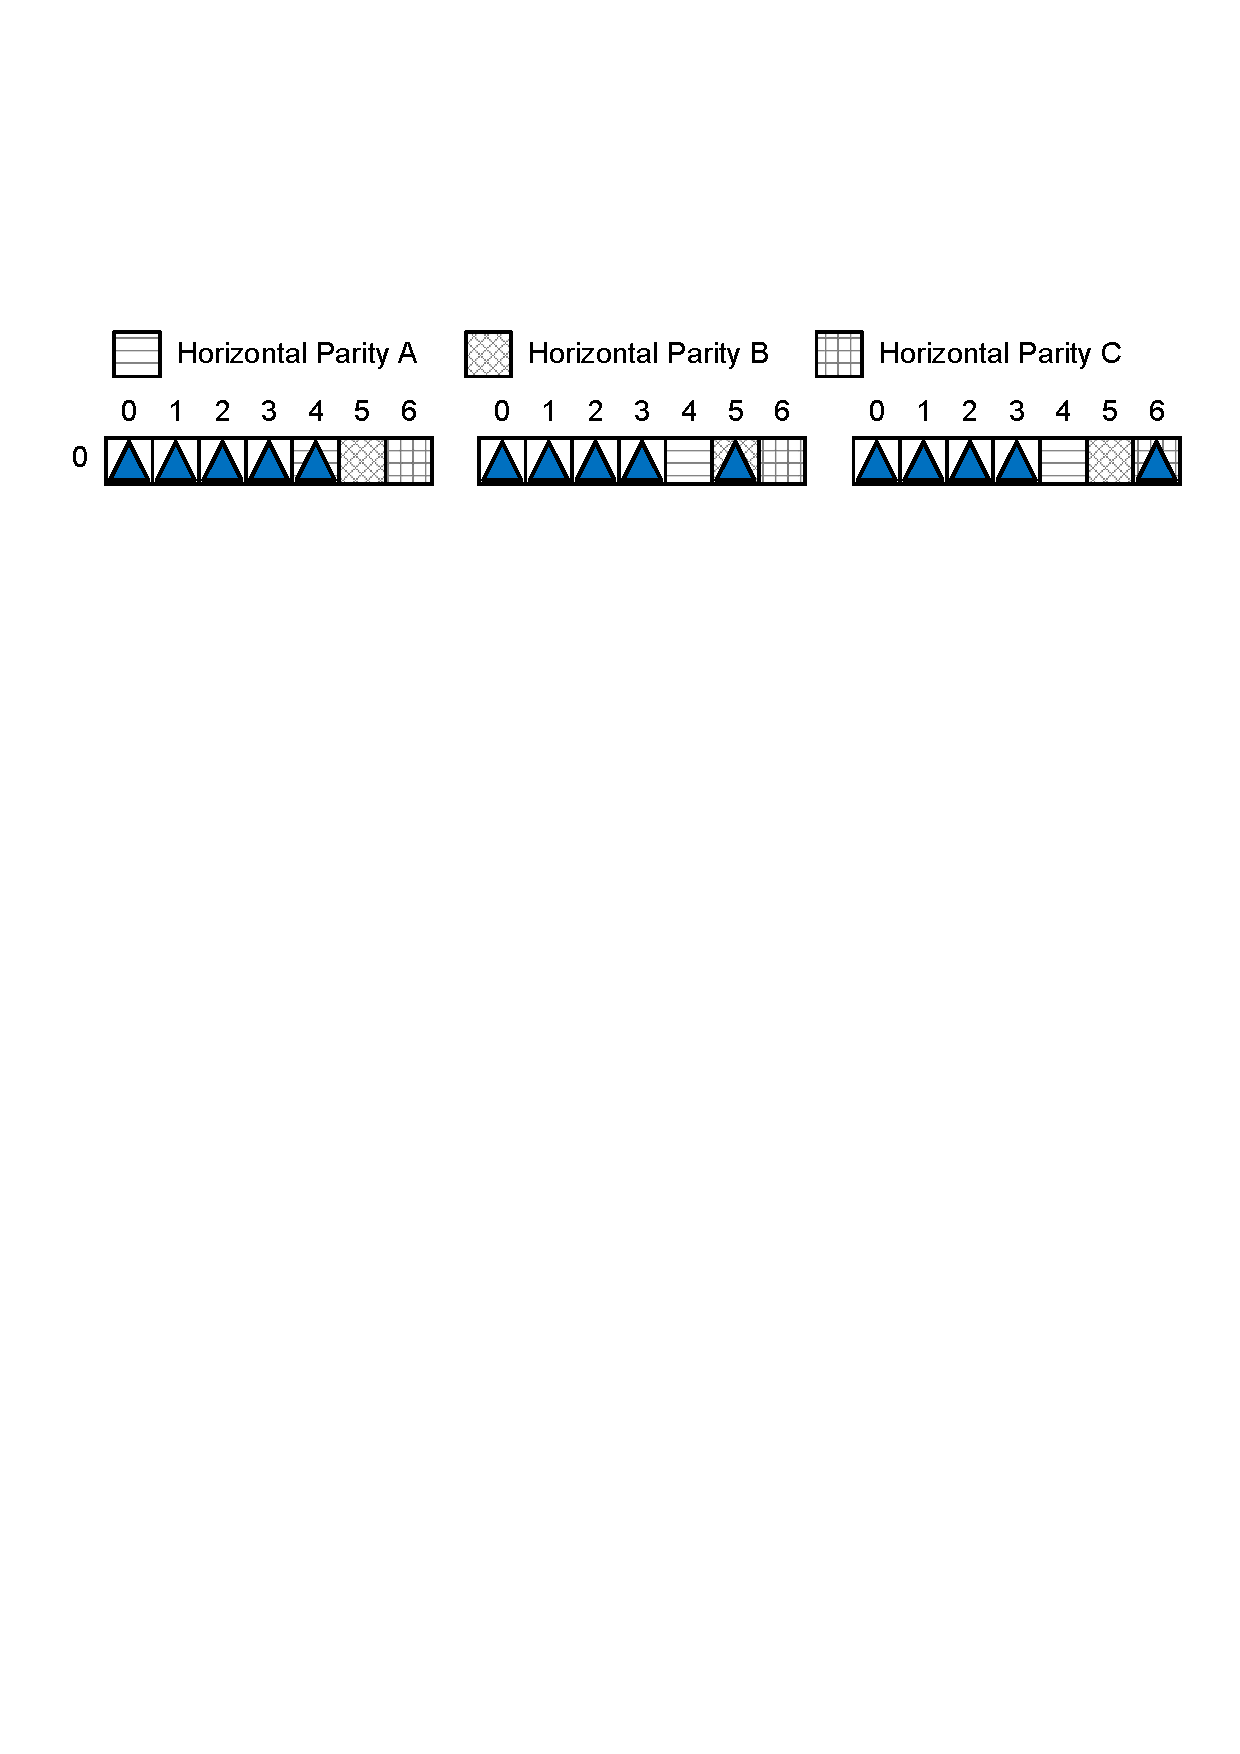
\includegraphics[width=0.92\linewidth]{photo/RS-1.pdf}\label{fig-RS-1}
}
\subfigure[\textbf{LRC Code} for arbitrary storage nodes ($k=4, r=2, g=2$), where 4 nodes are divided into 2 local groups (node 0-1 and node 2-3) and each of them has a local parity. The figure shows the encoding of local and global parities. (e.g., the local parity $C_{0,5} = \sum_{i=2}^3 A_{0,i}C_{0,i}$ and the global parity $C_{0,7} = \sum_{i=0}^3 A_{0,i}C_{0,i}$)]{
    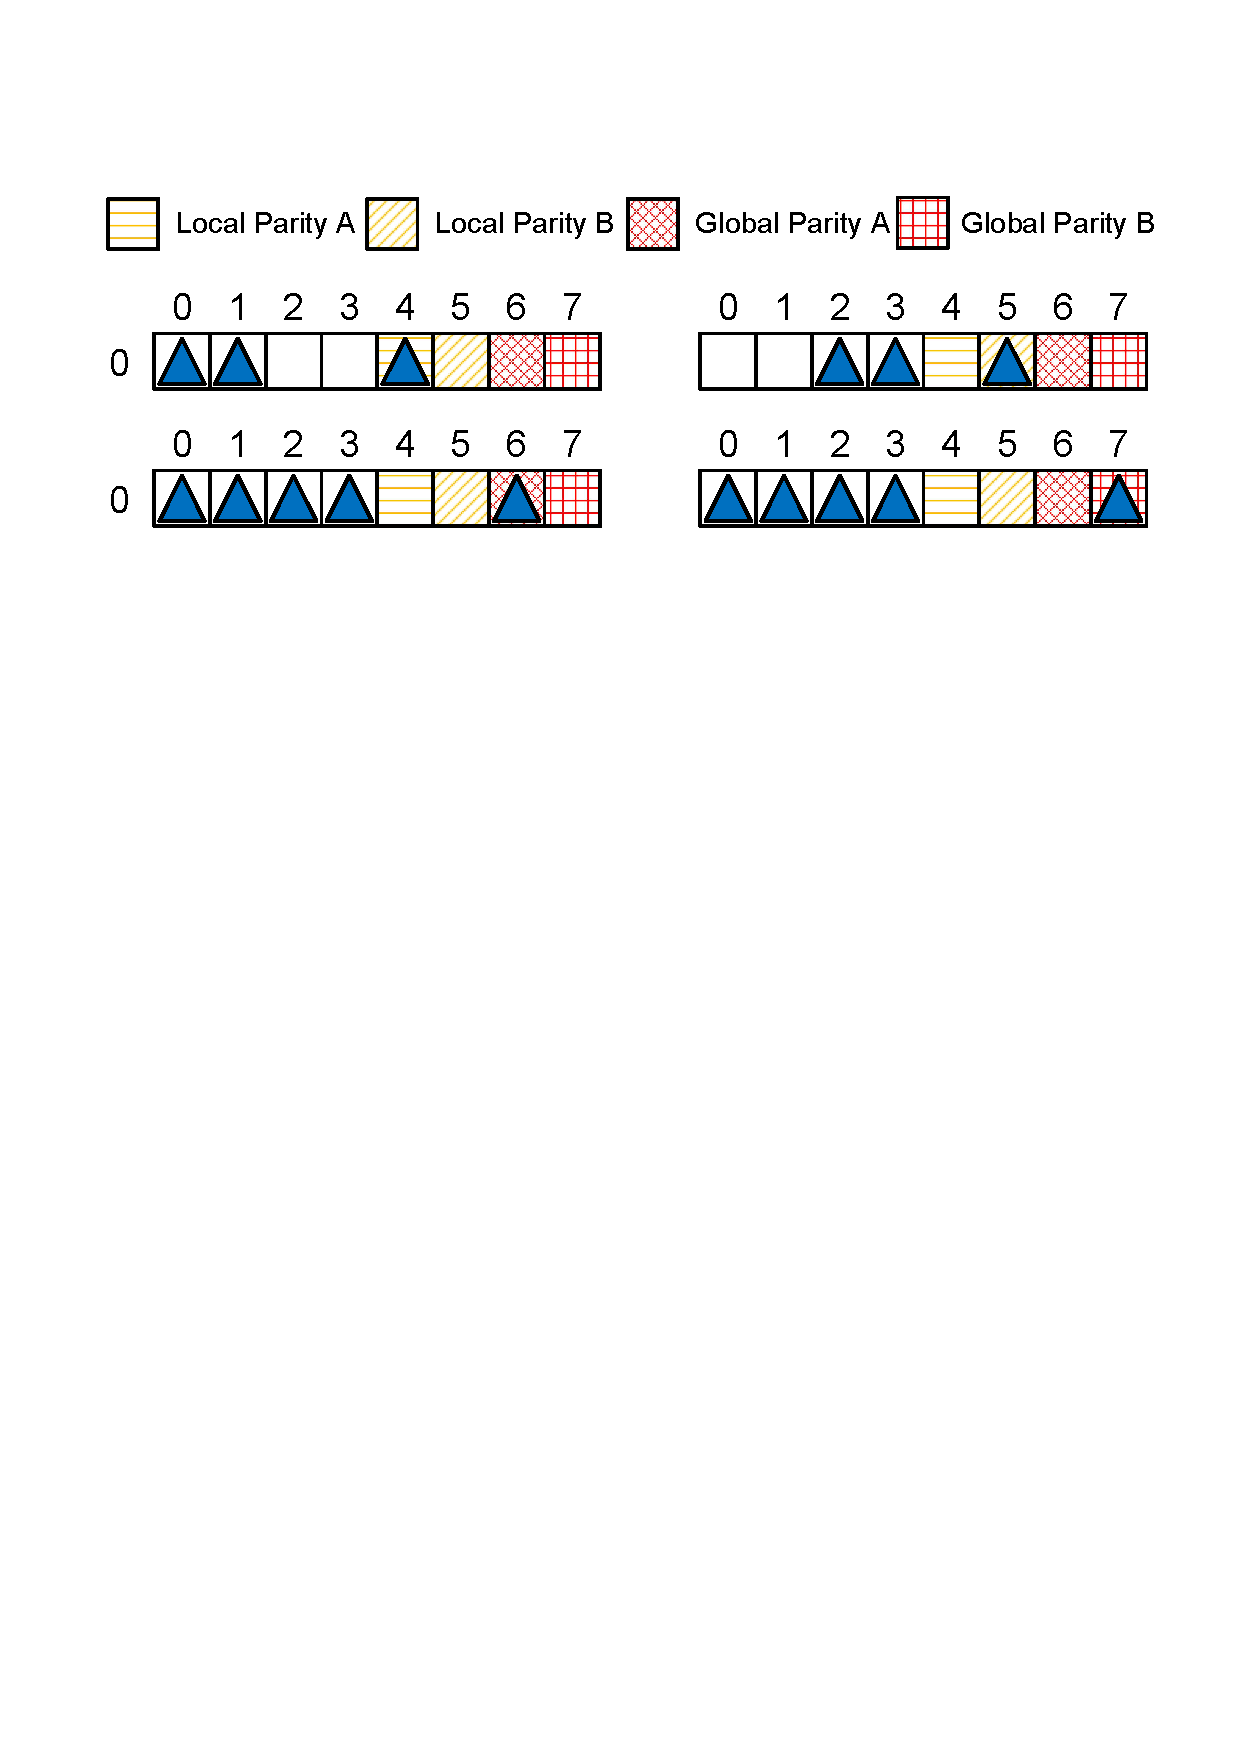
\includegraphics[width=0.8\linewidth]{photo/LRC-1.pdf}\label{fig-LRC-1}
}
\caption{Encoding of RS codes and LRC.}
\end{figure}

STAR code \cite{STAR} is an extension of EVENODD \cite{EVENODD} code, as shown in Figure \ref{fig-star}.
In the encoding process of STAR code, the generation of diagonal parity and anti-diagonal parity requires to calculate $S1$ and $S2$ first, which leads to a long parity chain.

\begin{figure}[ht]
\centering
\subfigure[\textbf{STAR Code:} For example, in the diagonal parity $S = C_{3,1} \oplus C_{2,2} \oplus C_{1,3} \oplus C_{0,4}$ and $C_{0,6} = C_{0,0} \oplus C_{3,2} \oplus C_{2,3} \oplus C_{1,4} \oplus S$.]{
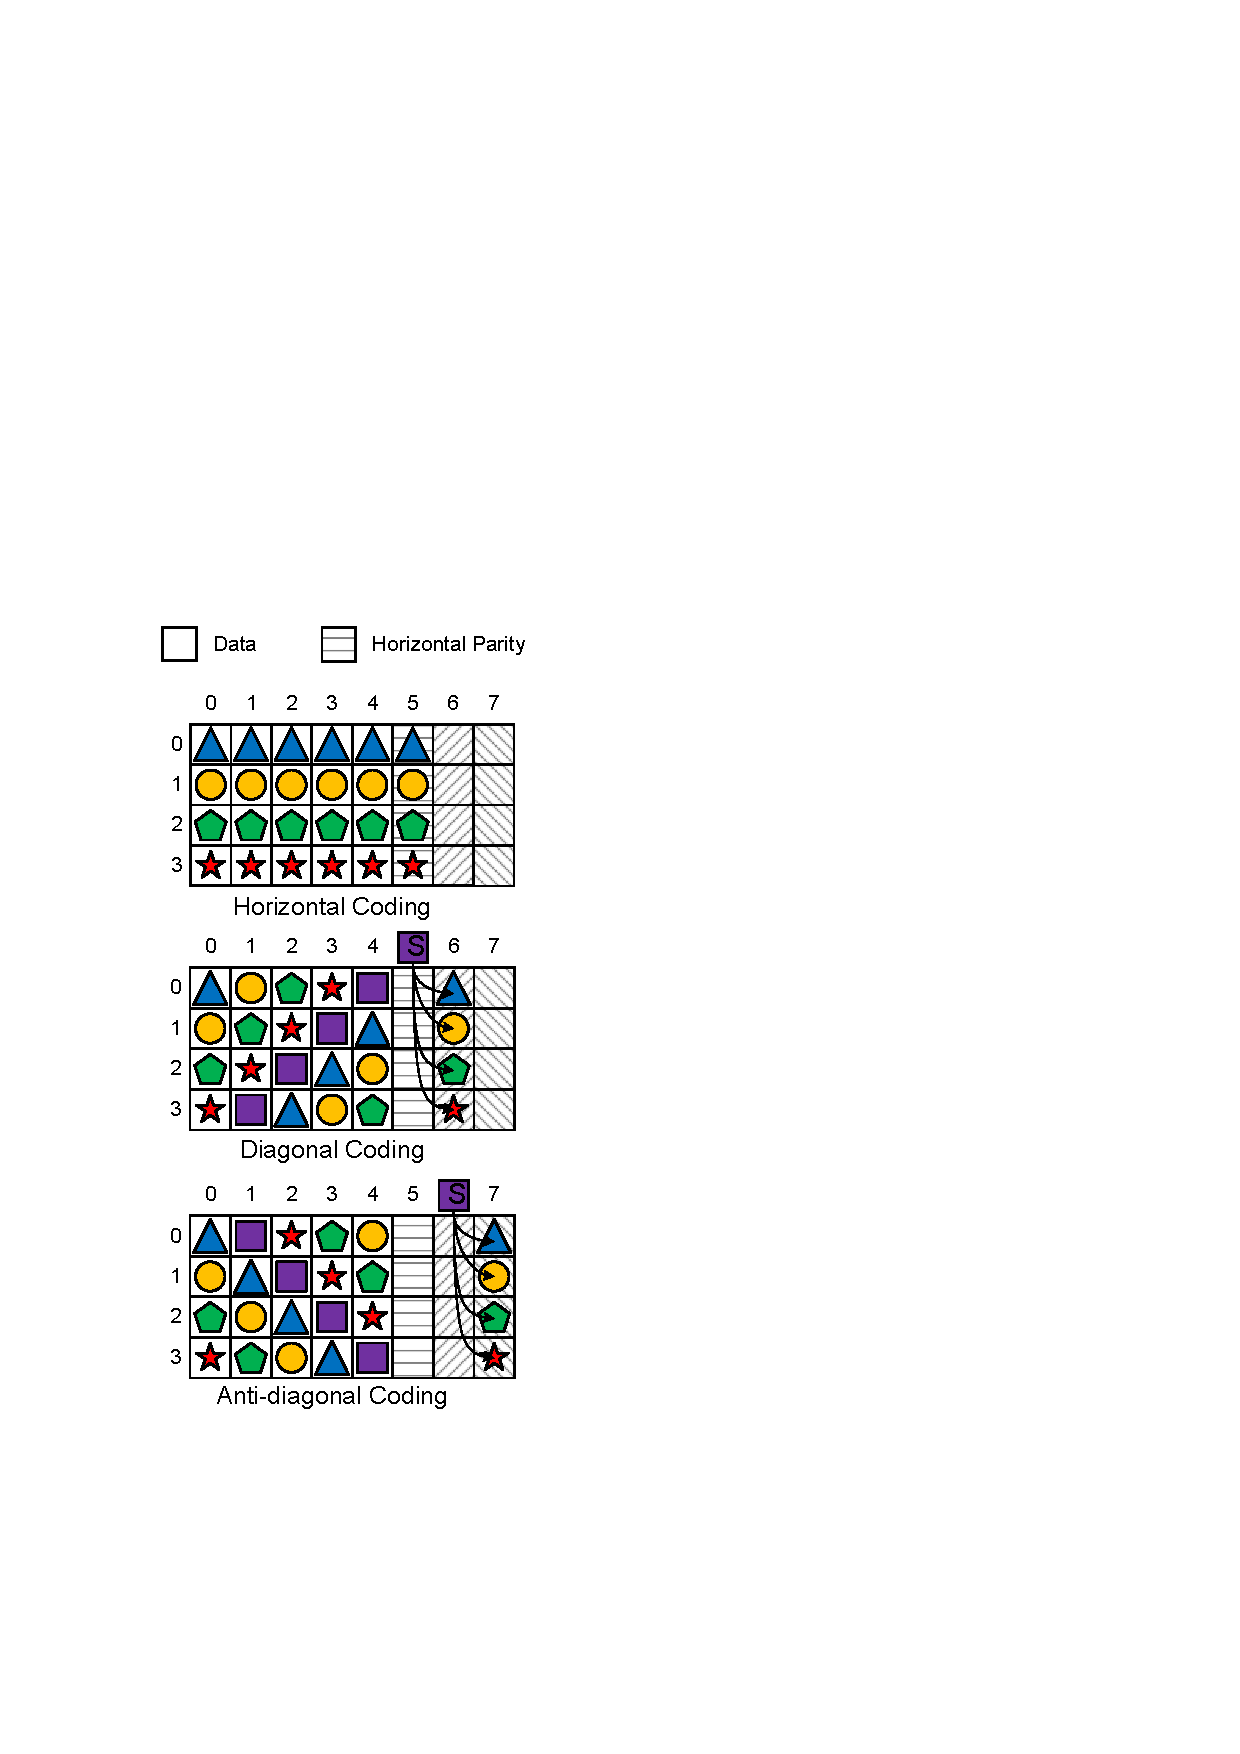
\includegraphics[height=6.3cm]{photo/STAR.pdf}\label{fig-star}
}
\hspace{6pt}
\subfigure[\textbf{TIP-Code:} For example, in the horizontal parity $C_{0,5} = C_{0,0} \oplus C_{0,2} \oplus C_{0,3}$]{
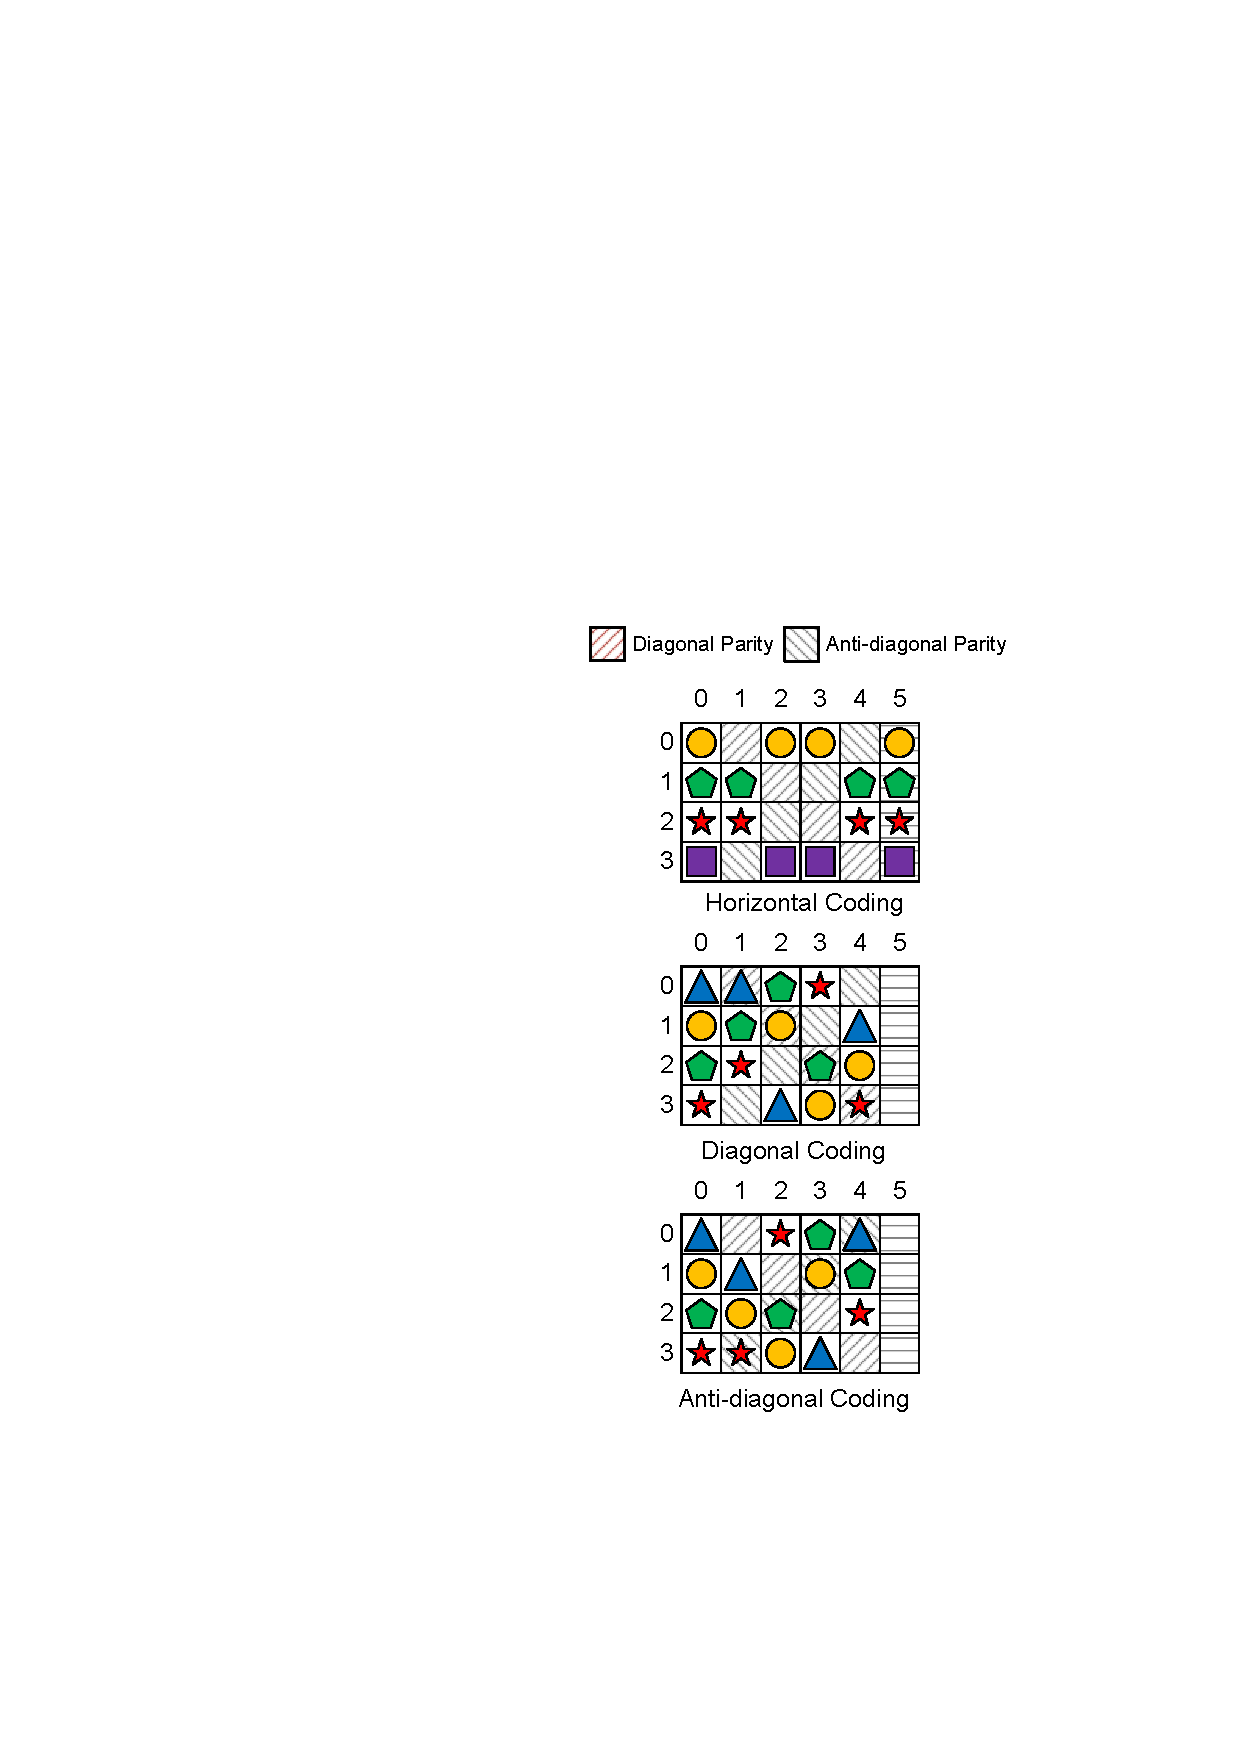
\includegraphics[height=6.3cm]{photo/TIP.pdf}\label{fig-TIP}
}
\caption{\small{Encoding of STAR ($p = 5$) (Figure \ref{fig-star}) and TIP ($p = 3$) (Figure \ref{fig-TIP}) codes. Each column represents a node, each block represents an element, and parity chains are represented by elements with same shape. STAR requires the number of data nodes to be $p$, and TIP requires that to be $p-2$.}}

\label{fig-star-TIP}
\end{figure}

TIP-Code\cite{TIP} is also an XOR-based 3DFTs erasure code, as shown in Figure \ref{fig-TIP}.
Compared with STAR code, the parities are generated independently, which reduces the number of I/O operations for partial stripe writes.

\subsection{Approximate Storage}
Approximate storage is an innovative approach for storage devices \cite{zhao2017approximate, sampson2014approximate, guo2016high, jevdjic2017approximate}, which enables applications to store data approximately. It can improve the performance, lifetime, or reduce the power consumption of different storage devices.

Specifically, for video applications, there are several approximate storage methods \cite{guo2016high, jevdjic2017approximate} for bit-level reliability in progressively encoded multimedia data.  \cite{guo2016high} identifies the relative importance of the encoded bits on the image quality and applys different levels of error correction. \cite{jevdjic2017approximate} shows how reliability of video storage can be traded for density and achieves the optimal quality/density points by tracking visual and metadata dependencies within the encoded bit stream.


\begin{table}[ht]\footnotesize
\centering
\caption{
Comparison of storage overhead, fault tolerance and computing overhead among various storage methods for video files.}\label{tab-AS-EC-AP}
\begin{tabular}{|c|c|c|c|c|}
\hline
\multirow{2}{*}{Schemes} & \multirow{2}{*}{Layer} & Storage & Fault & Computing \\
 &  & Overhead & Tolerance & Overhead \\ \hline
Data& Application & \multirow{2}{*}{low} & \multirow{2}{*}{/} & \multirow{2}{*}{high} \\
Compression & Level &  &  &  \\ \hline
RS-based EC & \multirow{10}{*}{\begin{tabular}[c]{@{}c@{}}Device\\ Level\end{tabular}} & \multirow{2}{*}{high} & \multirow{2}{*}{high} & \multirow{2}{*}{high} \\
for 3DFTs &  &  &  &  \\ \cline{1-1} \cline{3-5} 
XOR-based EC &  & \multirow{2}{*}{high} & \multirow{2}{*}{high} & \multirow{2}{*}{low} \\
for 3DFTs &  &  &  &  \\ \cline{1-1} \cline{3-5} 
RAID-6 &  & medium & medium & low \\ \cline{1-1} \cline{3-5} 
RAID-5 &  & low & low & low \\ \cline{1-1} \cline{3-5} 
Approximate &  & \multirow{2}{*}{very low} & \multirow{2}{*}{very low} & \multirow{2}{*}{low} \\
Storage &  &  &  &  \\ \cline{1-1} \cline{3-5} 
Approximate &  & \multirow{2}{*}{low} & \multirow{2}{*}{high} & \multirow{2}{*}{low} \\
Code &  &  &  &  \\ \hline
\end{tabular}
\end{table}

\subsection{Our Motivation}
We summarize various methods to reduce storage cost for video files in Table \ref{tab-AS-EC-AP}, the device level scheme of existing 3DFTs has high storage overhead, while RAID-5 or RAID-6 maintains medium storage overhead but sacrifices fault tolerance. Although approximate storage achieves low cost, its reliability cannot satisfy cloud environment. Application layer methods such as compression algorithms have high computational overhead and need to be used together with erasure codes to ensure reliability.
Therefore, the existing solutions cannot guarantee high reliability and low overhead at the same time of video storage.

From the summary of Table \ref{tab-AS-EC-AP}, existing solutions have their drawbacks on providing high reliability with low storage cost. 
A feasible solution is combining various erasure codes with tiered storage \cite{krish2014hats} \cite{wang2014balancing} \cite{zhang2010automated} \cite{udipi2012lot}, which motivates us to propose Approximate Code.

\begin{figure*}[ht]
\centering
\includegraphics[width=0.83\linewidth]{photo/Framework-v3.pdf}
\caption{The Framework of Approximate Code.}\label{fig-framework}
\end{figure*}

\section{Approximate Code}\label{ApCode}
In this section, we introduce the Approximate Code Framework and its properties through a few simple examples.

\subsection{Overview of Approximate Code Framework}
The Approximate Code Framework contains four main steps, code input, code segmentation, structure selection and code generation, as shown in Figure \ref{fig-framework}.

\subsubsection{Code Input}
Acquire an erasure coding input and get the corresponding parameters. Typically, for cloud storage systems, erasure codes used in 3DFTs are all accepted as the input. Several parameters related to erasure codes need to be collected, such as the number of data nodes $k$ and the number of parity nodes $r$.

\subsubsection{Code Segmentation}
For an inputted erasure code, we assume that its fault tolerance is $x$. The Approximate Code first splits its parities into two parts, local and global parities. The local parities are used for all data, while the global parities focus on the important data. Code segmentation are designed to ensure that local parities can tolerate any $r$ node failures, so the fault tolerance of unimportant data is $r$. For important data, the code segmentation ensures that the important data have the capabilities of fault tolerance by up to $x$ nodes.

For example, several erasure codes in 3DFTs like STAR have three types of parities, horizontal, diagonal and anti-diagonal parities. In the code segmentation step, the horizontal parities are regarded as local parities, which are separated from the diagonal/anti-diagonal parities (shown in Fig. \ref{fig-ap-STAR} and illustrated in Section \ref{APPRXOR} in detail).

\subsubsection{Structure Selection}
The framework chooses the structure after code segmentation.
There are two main structures for distributing the important and unimportant data, as shown in Figure \ref{fig-framework}. In Even Structure, important data are distributed uniformly among all data nodes, while in Uneven Structure, they are stored among several nodes dedicatedly.
%We specify that in Even Structure, the ratio of important data to each node is $1/h$, thereby ensuring that the number of important data in both Even Structure and Uneven Structure just fills up $k$ nodes.

Since Even Structure distributes the important data across each node, it guarantees a balanced workload. Meanwhile, Uneven Structure aggregates important data into several dedicated nodes, which provides better reliability (illustrated in Section \ref{ReconstructionFT}).

\subsubsection{Code Generation}\label{code-gen}
After the code segmentation and structure selection, the Approximate Code Framework generates an approximate form of the inputted erasure code.
The construction of the Approximate Code is determined by four parameters ($k$, $r$, $g$, $h$) and the structure type.

We define the output Approximate Code as \textbf{APPR.CodeName ($k,r,g,h$, Structure Type)}, where ``CodeName'' is the name of the input erasure code. Structure type is Even or Uneven and the default configuration selects both two structures.

According to these parameters, Approximate Code Framework divides the data/parity nodes into several local stripes. Each local stripe has $n$ nodes,  
In an $n$-node stripe, $k$ of them are data nodes and $r=n-k$ nodes are local parity nodes.
We define that the ratio of important data is $1/h$, and the framework utilizes $h$ local stripes to construct a global stripe, which includes $k*h$ data nodes and $r*h$ local parity nodes in total.
In a global stripe, $g$ additional nodes are designed for global parities, which are calculated by the important data, so the total number of nodes in APPR.CodeName ($k,r,g,h$) is
$N= h*(k+r) + g$.

Approximate Code guarantees that the unimportant data can tolerate any $r$ node failures and the important data can tolerate any $r+g$ node failures if the inputted erasure code is an MDS code.
Since the 3DFTs is a typical configuration, we mainly discuss the situation of $r+g=3$ in the rest of our paper, so $r$ is usually $1$ or $2$.

\subsection{Approximate RS-based Codes}\label{appr-rsbased}
RS-based codes are based on the calculation of Galois Field (GF), which are designed for arbitrary number of data nodes. Therefore, in the code segmentation step of  Approximate Code Framework, we divide the RS-based codes into two parts, $r$ parties and $g$ parities. In the structure selection step, the important data can be distributed in both two structures. Here we take RS and LRC codes to show how Approximate Code Framework works.

\subsubsection{Approximate RS Code (APPR.RS)}
We consider RS($4,3$) as the inputted erasure code, as shown in Figure \ref{fig-RS-2}. Three horizontal parities are divided into one local and two global parities with the Uneven Structure, and finally we generate APPR.RS ($4,1,2,3$,Uneven).
As a result, the unimportant data and their corresponding parities constitute a RS ($4,1$) array, and the important data and their corresponding parities form a RS ($4,3$).

\begin{figure}
\centering
\subfigure[The structure of APPR.RS ($4,1,2,3$,Uneven) ]{
    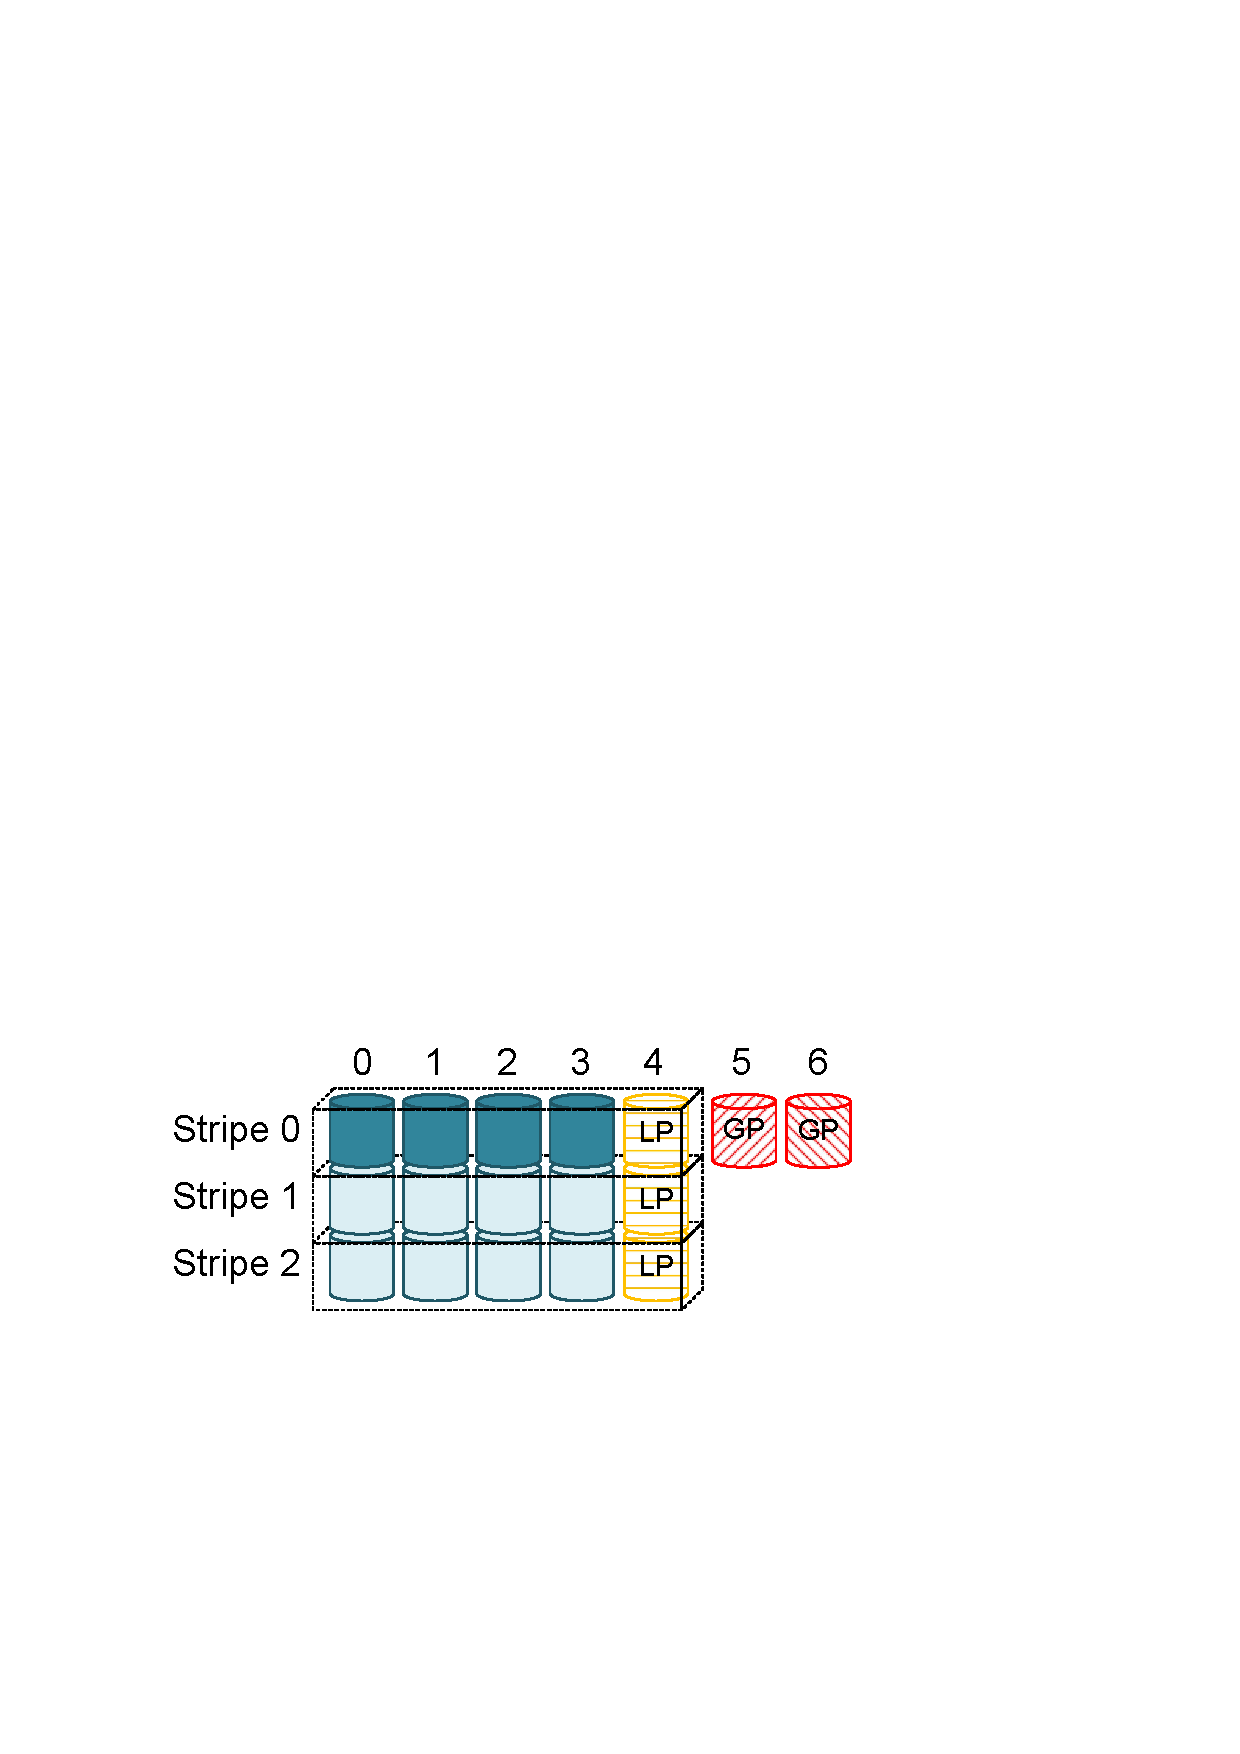
\includegraphics[width=0.42\linewidth]{photo/RS-3.pdf}\label{fig-RS-3}
}\hspace{3mm}
\subfigure[The structure of APPR.LRC ($4,2,2,3$,Even)]{
    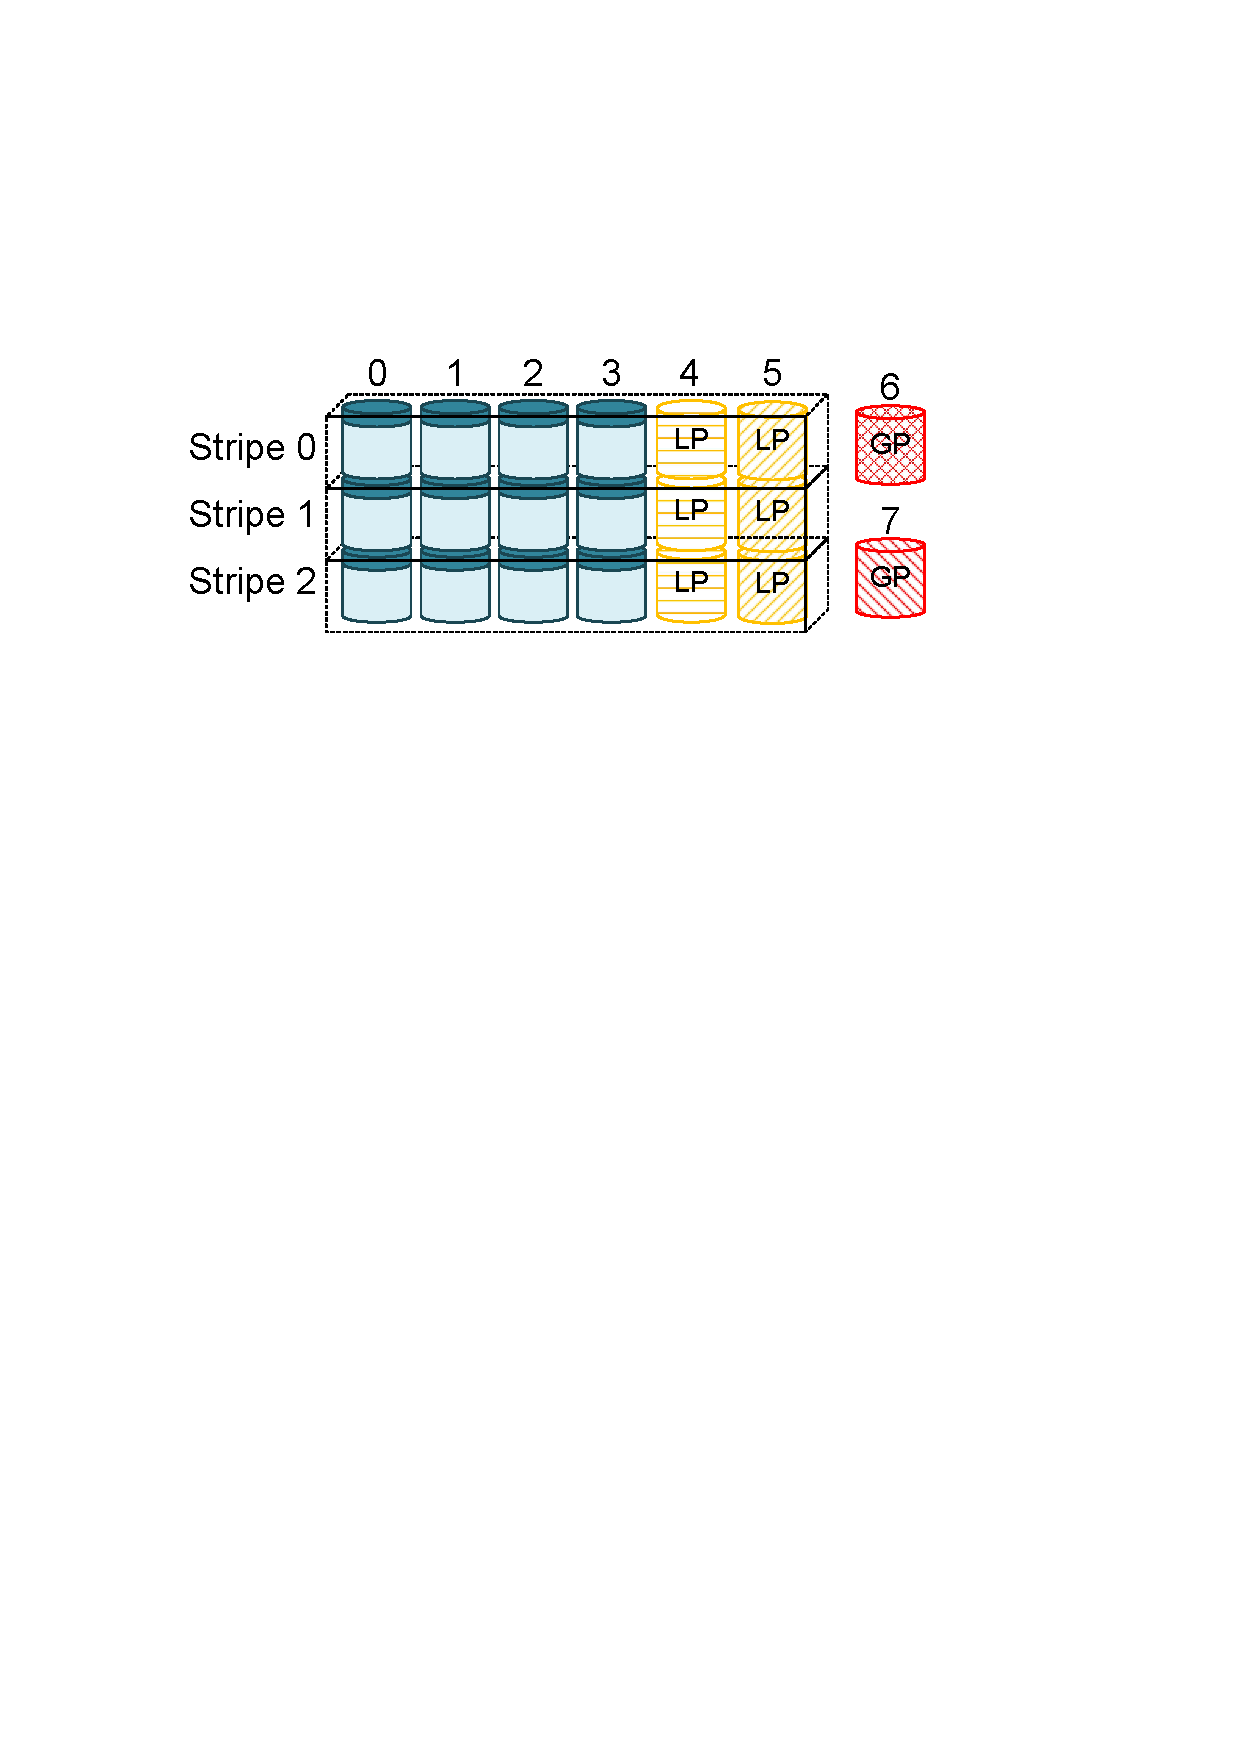
\includegraphics[width=0.42\linewidth]{photo/LRC-3.pdf}\label{fig-LRC-3}
}

\subfigure[The generation of APPR.RS ($4,1,2,3$,Uneven) ]{
    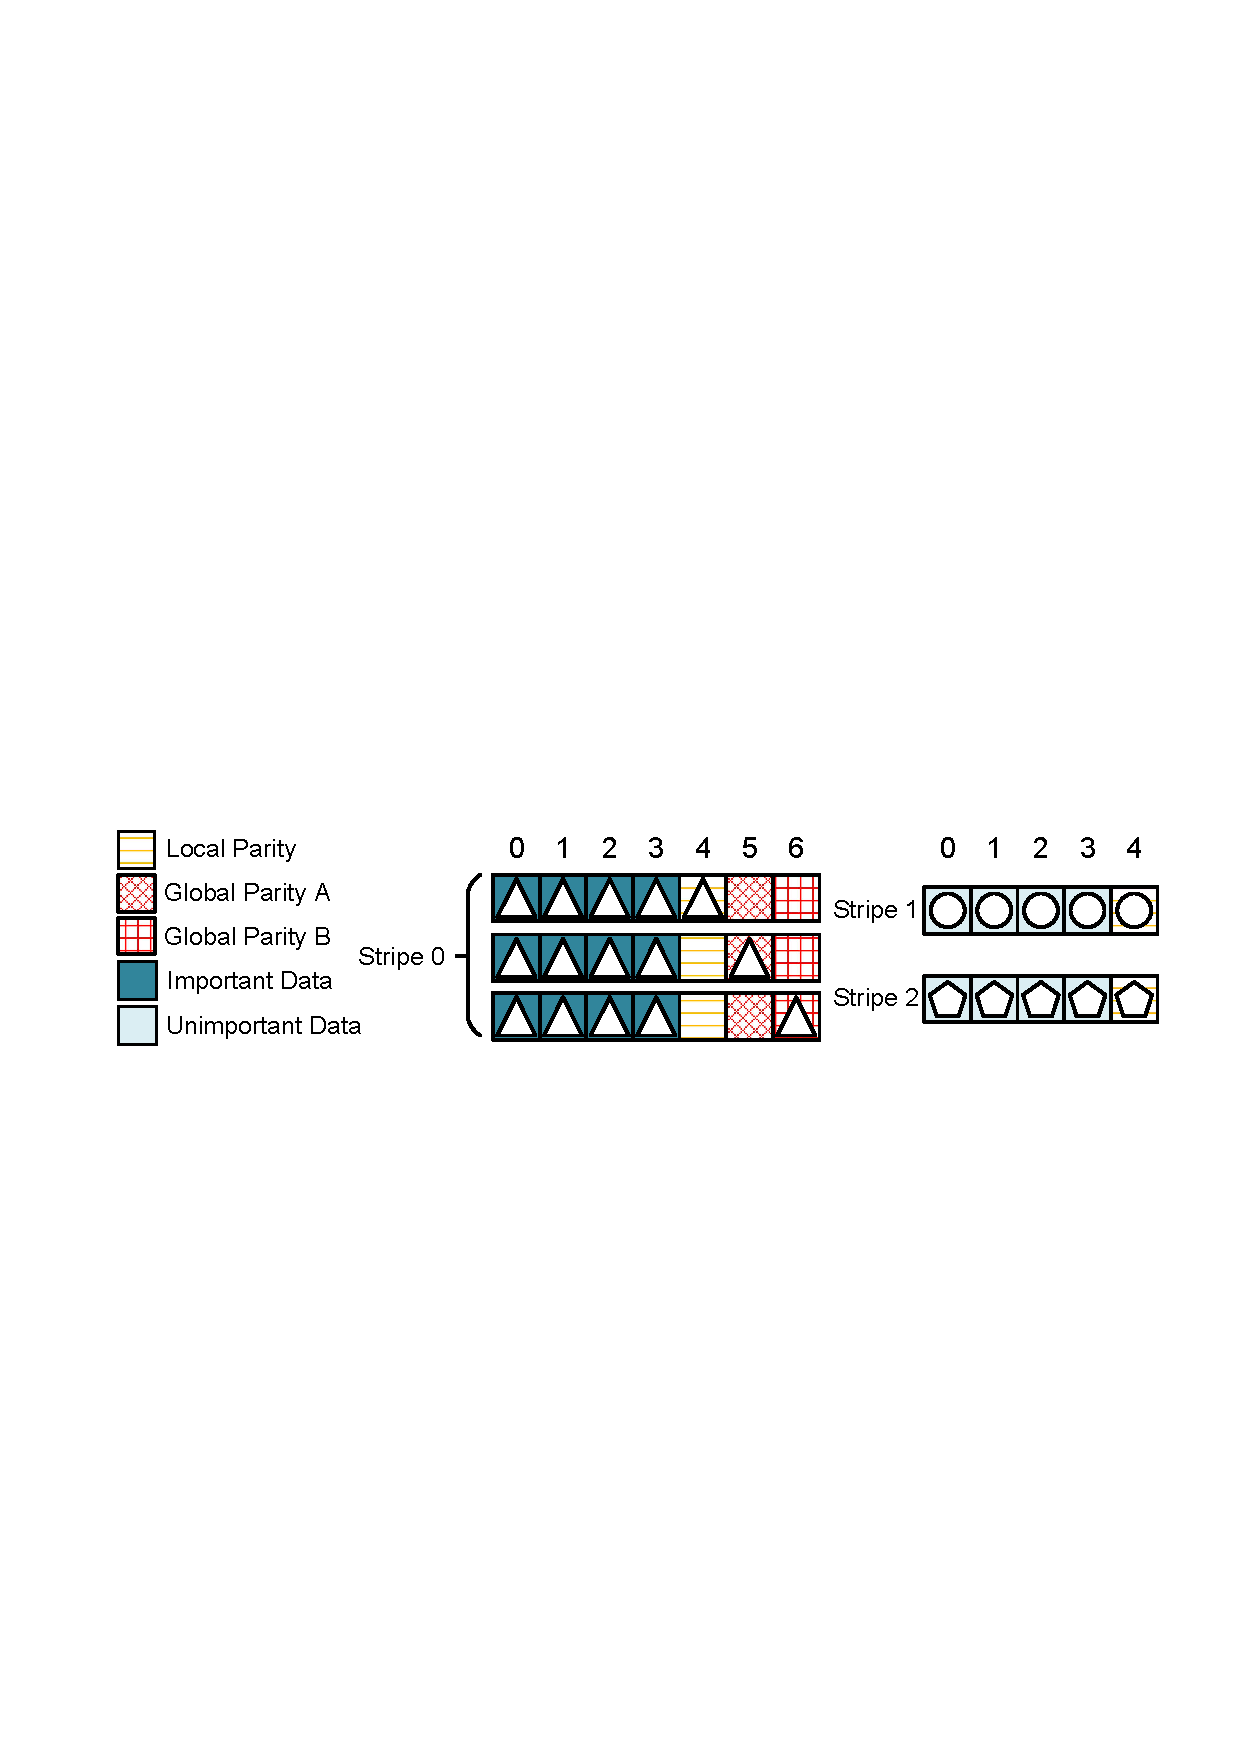
\includegraphics[width=0.85\linewidth]{photo/RS-2.pdf}\label{fig-RS-2}
}
\subfigure[The generation of APPR.LRC ($4,2,2,3$,Even)]{
    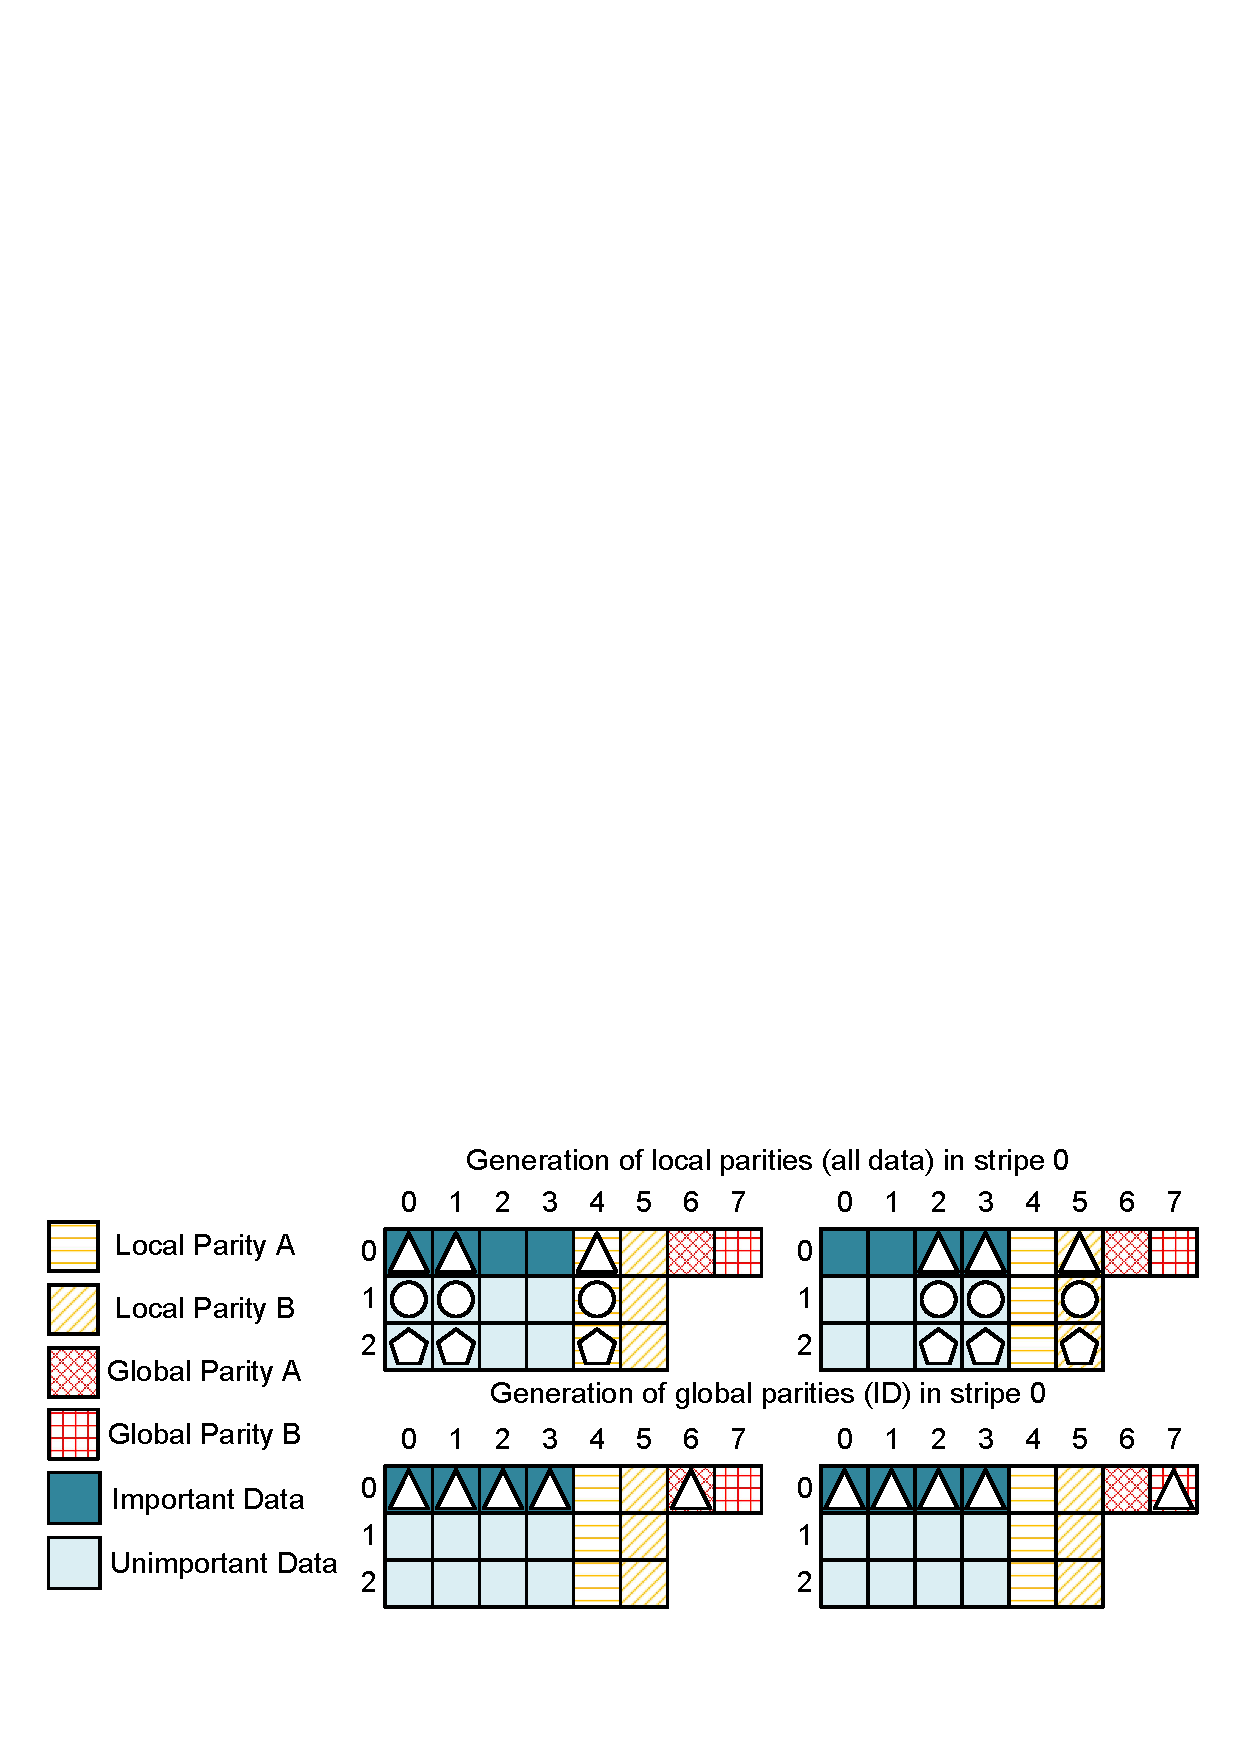
\includegraphics[width=0.85\linewidth]{photo/LRC-2.pdf}\label{fig-LRC-2}
}
\caption{Construction of APPR.RS and APPR.LRC codes via Approximate Code Framework.}
\end{figure}

\subsubsection{Approximate LRC (APPR.LRC)}

We take LRC ($4, 2, 2$) \cite{LRC} as an example (shown in Figure \ref{fig-LRC-2}), which means
that two local parities and two global parities are generated initially. Similar to the construction of RS code, the global parities are generated only by the important data. At last we get the APPR.LRC ($4, 2, 2, 3$, Even)\footnote{Since LRC code is not an MDS erasure code, the fault tolerance of APPR.LRC ($4, 2, 2, 3$) is the same as APPR.RS ($4,1,2,3$)}.

\subsection{Approximate XOR-based Codes}\label{APPRXOR}
Since we mainly provide 3DFTs for important data, we prefer to construct Approximate Code with several XOR-based codes to provide faster encoding/decoding speed than RS-based codes. Here we introduce two typical constructions of Approximate XOR-based codes, Approximate STAR Code and Approximate TIP-Code.

\subsubsection{Approximate STAR Code (APPR.STAR)}

As introduced in Section \ref{existEC}, STAR Code \cite{STAR} is a typical XOR-based erasure code for 3DFTs, which is a direct extension of EVENODD\cite{EVENODD} (RAID-6 code) by adding the anti-diagonal parities. Figure \ref{fig-ap-STAR} shows the construction of APPR.STAR ($5,2,1,4$,Uneven). In this case, the horizontal and diagonal parities are regarded as local parities,  the anti-diagonal parities are defined as global parities in Approximate Code Framework.

Briefly, according to the construction of APPR.STAR ($5,2,1,4$, Uneven), the important data are encoded by STAR code while the unimportant data are generated by EVENODD code. It is clear that the important/unimportant data can tolerate triple/double nodes fail, respectively.

\begin{figure}[ht]
\centering
\subfigure[Structure selection.]{
    \label{fig-ap-STAR-str}
    \includegraphics[width = 0.4\linewidth]{photo/APPR-STAR-STR.pdf}
}

\subfigure[Generation of APPR.STAR.]{
    \label{fig-ap-STAR-GEN}
    \includegraphics[width = 0.85\linewidth]{photo/APPR-STAR-GEN.pdf}
}

\caption{Construction of APPR.STAR  ($5,2,1,4$,Uneven) via Approximate Code Framework.}\label{fig-ap-STAR}
\end{figure}


\begin{figure}[ht]
\centering
\subfigure[Structure selection of APPR.TIP-Code]{
    \label{fig-ap-TIP-a}
    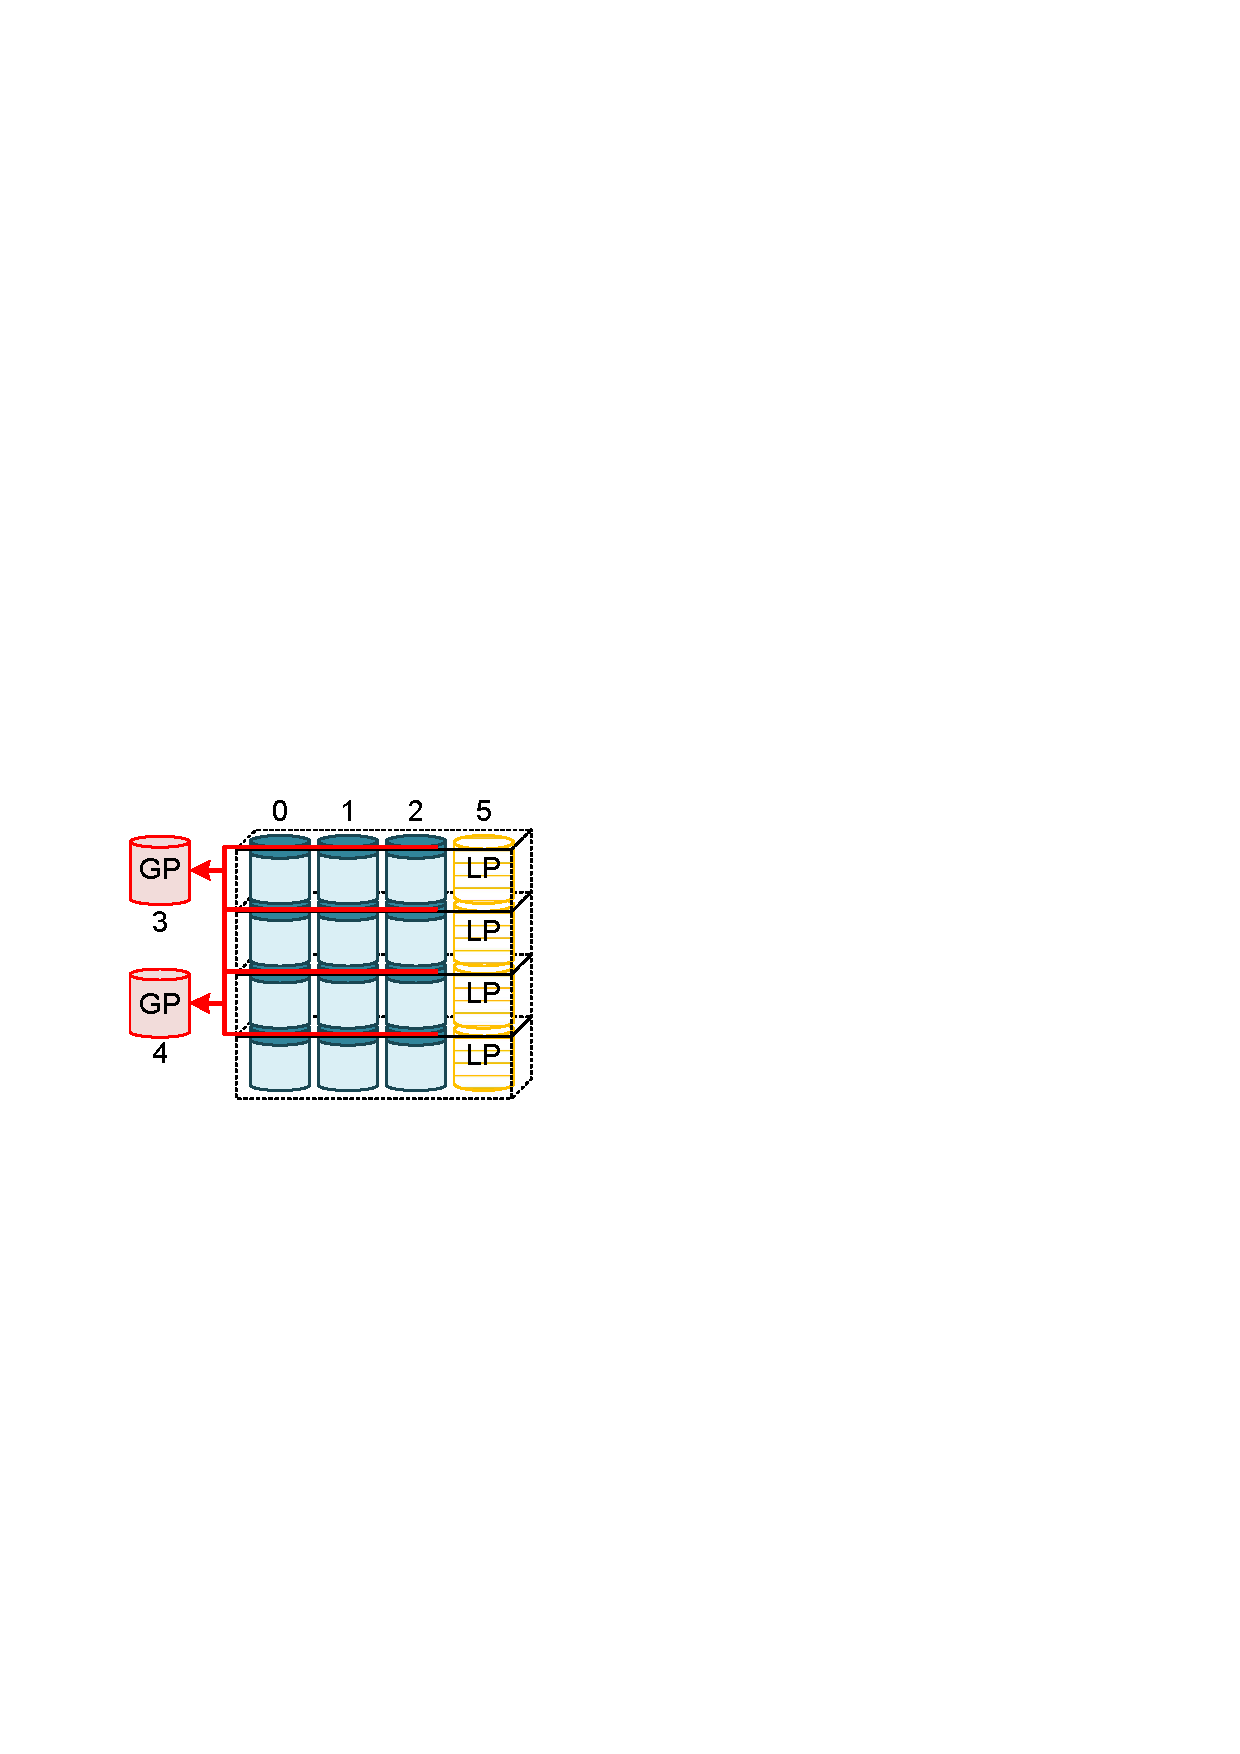
\includegraphics[width = 0.4\linewidth]{photo/TIP-a.pdf}
}
\hspace{5pt}
\subfigure[Generation of local parities]{
    \label{fig-ap-TIP-b}
    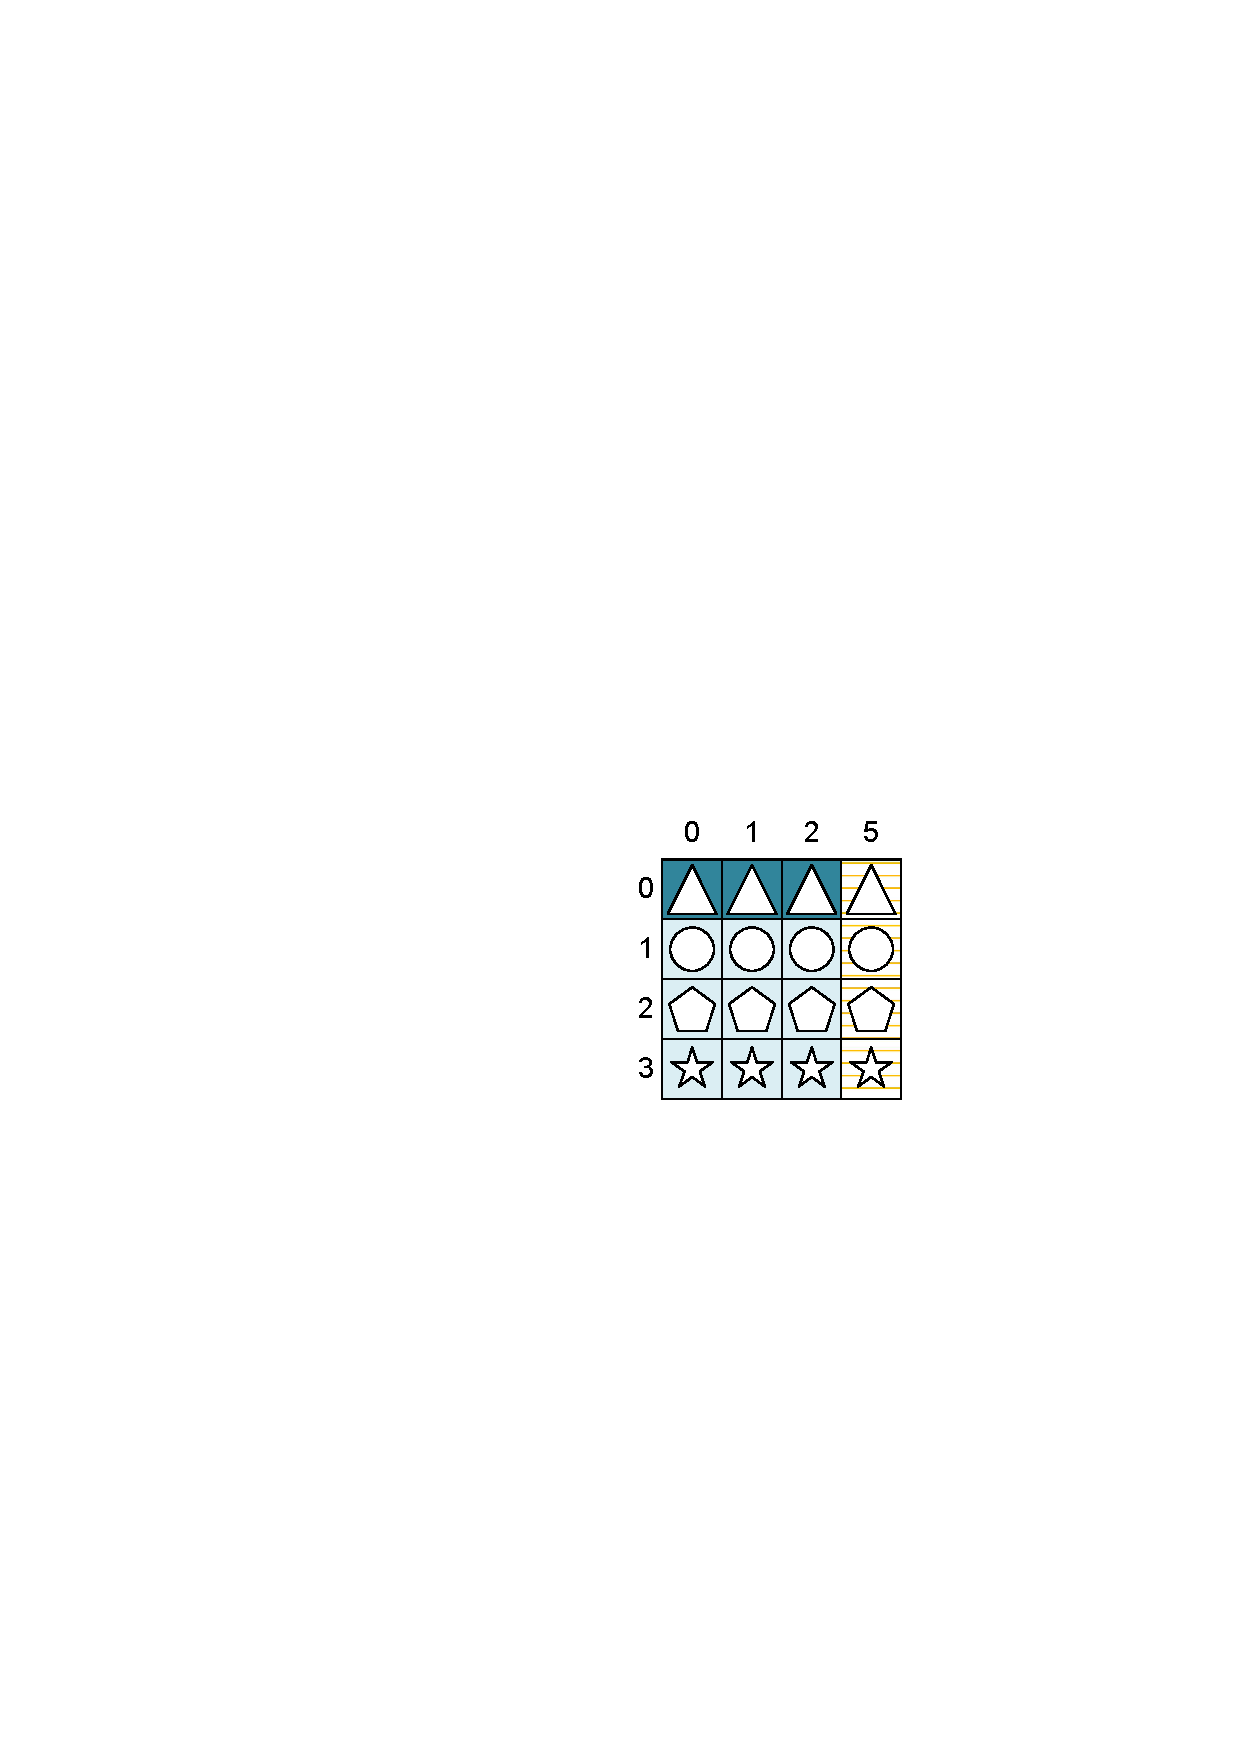
\includegraphics[width = 0.3\linewidth]{photo/TIP-b.pdf}
}

\subfigure[Generation of global parities]{
    \label{fig-ap-TIP-c}
    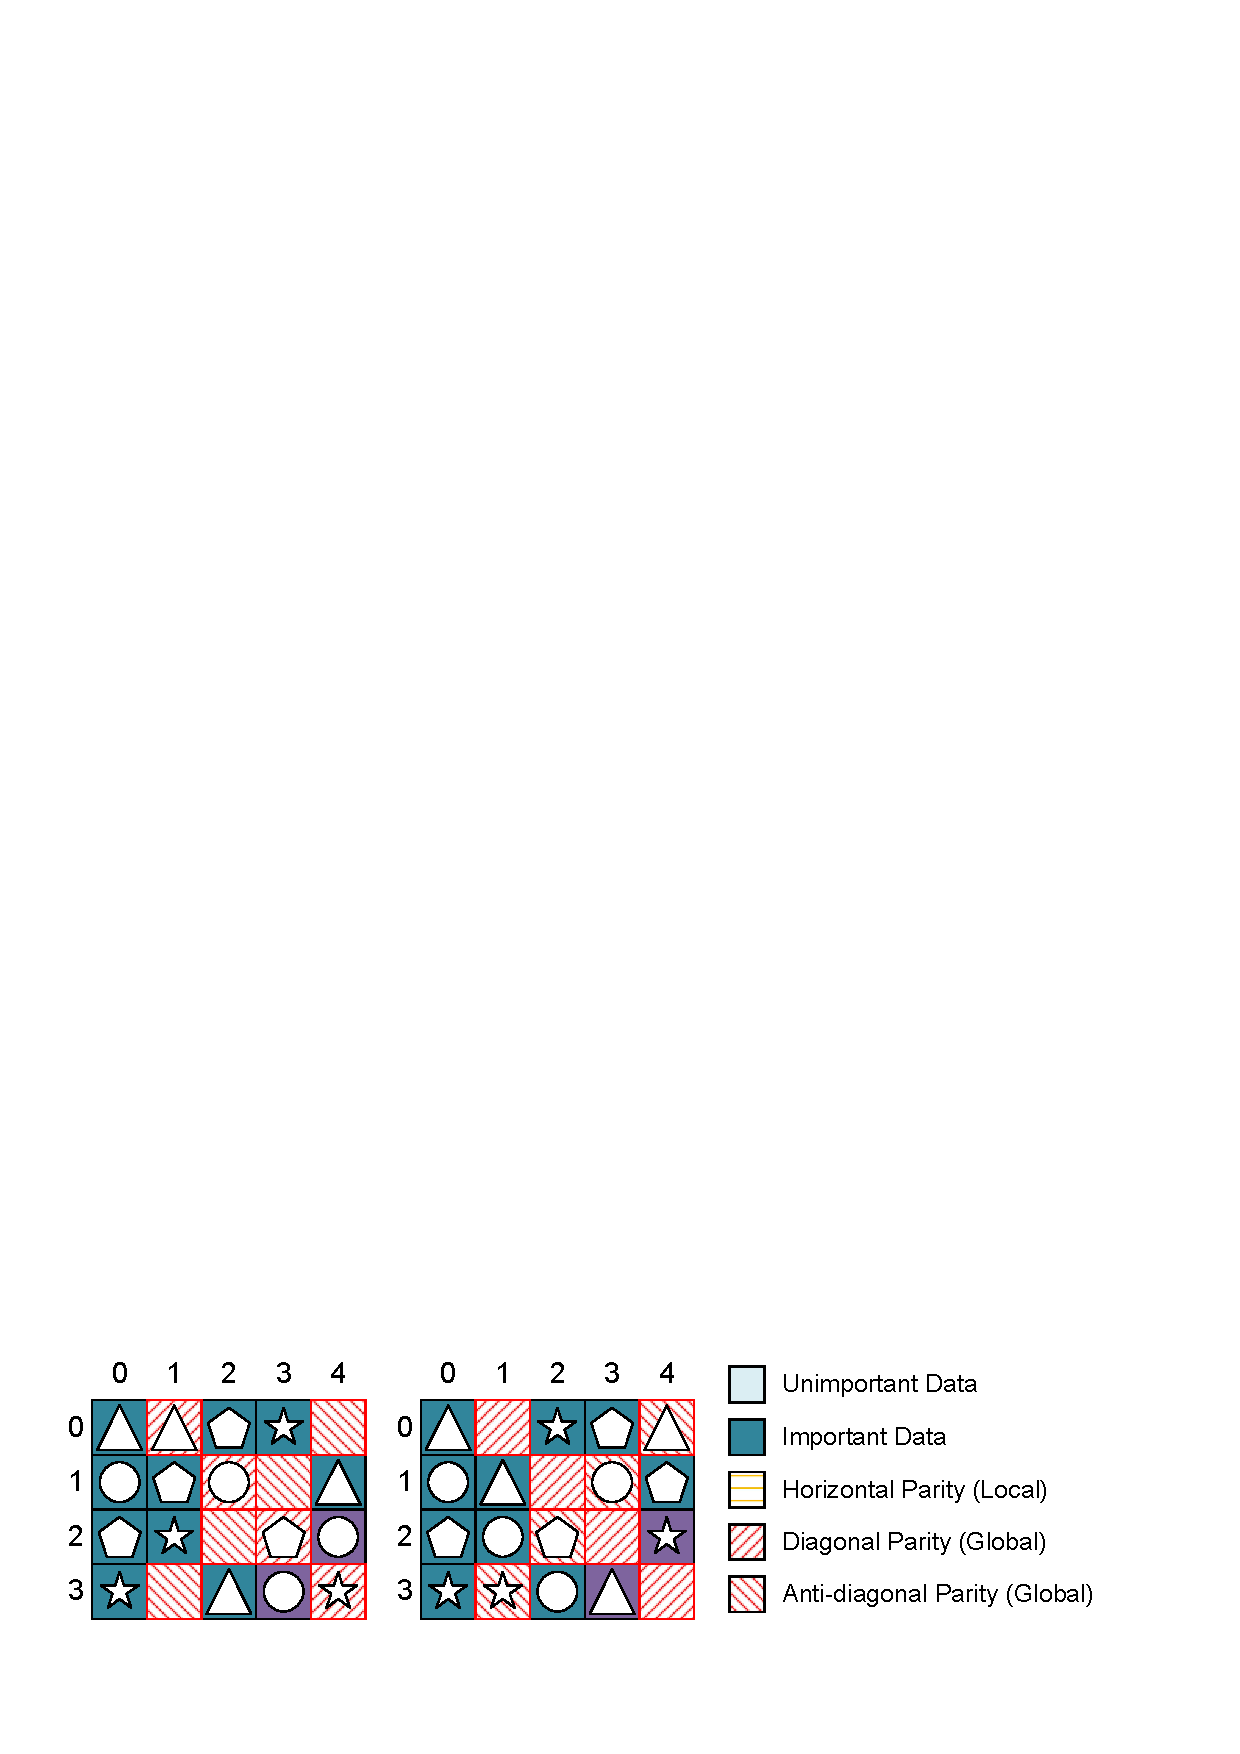
\includegraphics[width = 0.85\linewidth]{photo/TIP-c.pdf}
}

\caption{The construction and the encoding process of APPR.TIP ($3,1,2,4$,Even). The node 3 and 4 in TIP-Code are defined as the global parity nodes in this case.}\label{fig-ap-TIP}

\end{figure}

\subsubsection{Approximate TIP-Code (APPR.TIP)}

We use the generation of APPR.TIP ($3,1,2,4$,Even) as an example (shown in Figure \ref{fig-ap-TIP}). In the code segmentation phase, we split TIP-Code into two parts, the horizontal parity part, and the diagonal/anti-diagonal parities part. The important data are arranged in an Even Structure. Since the parities of the TIP-Code are distributed among several nodes, the code generation process is different from APPR.STAR.

We first generate local parity nodes by the horizontal parities for all data. Then, we reorganize the important data to construct new global stripes, where the diagonal and anti-diagonal parities are used to encode the important data. The number of global stripes are based on the ratio of important data ($1/h$). Here $h=6$, which means that the framework utilizes the important data from six local stripes to generate one global stripe.


\subsection{Reconstruction Process and Fault Tolerance}\label{ReconstructionFT}
Existing work \cite{LRC} has demonstrated that when we have $r$ local parities and $g$ global parities, the capability of fault tolerance is at least $r+g$ in typical. Thus the reconstruction (less than $r+g$ nodes fail) of the framework is classified into two cases,

(1) When $f \leqslant r$, all data (both important and unimportant data) are reconstructed via local parities.

(2) When $f \leqslant r+g$, the important data are reconstructed via both local and global parities.

However, under some special cases, important/unimportant data are also recoverable when ($f>r+g$)/($f > r+1$).
Here we only consider two situations: $f=r+1$ and $f=r+g+1$, because the former just exceeds the fault tolerance of unimportant data so we calculate $P_U$, while the latter just exceeds the fault tolerance of important data so we calculate $P_I$.
 Since in this paper we focus on the 3DFTs, $r+g$ is set to 3.

\subsubsection{When $f=r+1$}
Under Even Structure, the unimportant data nodes are recoverable as long as $f \leqslant r$.
There are $\binom{N}{r+1}$ cases of loss of $r+1$ nodes and there are $h$ stripes in all. In each stripe, $\binom{k+r}{r+1}$ cases result in unrecoverable data.

Under Uneven Structure, only $h-1$ stripes contain unimportant data, so $P_{U}$ is
\begin{align}
    P_{U-Even} &= 1 - \frac{h \times \binom{k+r}{r+1}}{\binom{N}{r+1}}\\
    P_{U-Uneven} &= 1 - \frac{(h-1) \times \binom{k+r}{r+1}}{\binom{N}{r+1}}
\end{align}

\subsubsection{When $f=r+g+1$ ($f=4$)}
The number of cases that $f=4$ is $\binom{N}{4}$.
We calculate the total number of cases on losing the important data, which are based on the different losses of the global parity nodes. The results are as follows,
\begin{align}
    P_{I-Even} = 1 - h*&\frac{\sum_{i=0}^{g} {\binom{k+r}{4-i}*\binom{g}{i}} }{\binom{N}{4}}  (g=1,2)\\
    P_{I-Uneven} &= 1 - \frac{\binom{k+3}{4}}{\binom{N}{4}}
\end{align}

According to the above equations, for APPR.RS ($3,1,2,3$, Even), $80.21\%$ double failures cases are recoverable for unimportant data, and $95.50\%$ quad failures is recoverable for important data nodes. For APRR.RS ($3,1,2,3$, Uneven), $P_U=86.81\%$, $P_{I}=98.50\%$.

\subsection{Properties of Approximate Code}\label{properties}

We analyze the nature of the Approximate Code from the following aspects, and summarize the results shown in Table \ref{tab-properties}.
\begin{itemize}
    \item Low Storage Overhead. Approximate Code reduces storage overhead by approximating and tiered storage strategies for important/unimportant data. 
    \item Low Update Complexity. When one node is updated, Approximate Code needs to write $r$ local parity nodes and only $g/h$ global parity nodes, which are less than the inputted erasure codes.
    \item High reliability for important data. Important data can be recovered in all triple nodes failure and most quad nodes failure environment.
    \item High Flexibility. Approximate Code Framework can be applied with any erasure codes in 3DFTs, and various parameters can be set.
\end{itemize}

\begin{table}[htb]\footnotesize
\centering
\caption{Comparison of storage overhead, fault tolerance and average single write performance among typical erasure codes and their Approximate Codes.}\label{tab-properties}
\begin{tabular}{|c|c|c|c|}
\hline
\multirow{2}{*}{Erasure Coding} & Storage & Fault Tolerance & Avg. Single Write \\
 & Overhead & Capability & Overhead \\ \hline
RS($k,r$) & $(k+r)/k$ & $r$ & $r+1$ \\ \hline
LRC($k,l,r$) & $1+\frac{l+r}{k}$ & $r+1$ & $r+2$ \\ \hline
STAR($p$) & $(p+3)/p$ & $3$ & $6-\frac{4}{p}$ \\ \hline
TIP-code($p$) & $\frac{p+1}{P-2}$ & $3$ & 4 \\ \hline
APPR.LRC & \multirow{8}{*}{$\frac{(k+r)h+g}{kh}$} & \multirow{2}{*}{$1+g$} & \multirow{2}{*}{$2+\frac{g}{h}$} \\ 
($k,r,g,h$) &  &  &  \\ \cline{1-1} \cline{3-4} 
APPR.RS &  & \multirow{2}{*}{$r+g$} & \multirow{2}{*}{$1+r+\frac{g}{h}$} \\
($k,r,g,h$) &  &  &  \\ \cline{1-1} \cline{3-4} 
APPR.STAR &  & \multirow{2}{*}{3} & \multirow{2}{*}{$2\frac{k-h-1}{kh}+4$} \\
($k,2,1,h$) &  &  &  \\ \cline{1-1} \cline{3-4} 
APPR.TIP &  & \multirow{2}{*}{3} & \multirow{2}{*}{$2+\frac{2}{h}$} \\
($k,1,2,h$) &  &  &  \\ \hline
\end{tabular}
\end{table}


\subsection{Implementation in Storage Systems}\label{Implementation}

\begin{figure}[htb]
\centering
\includegraphics[width=0.75\linewidth]{photo/implementation-V2.pdf}
\caption{Overview of Approximate Storage Layer.}
\label{fig-implementation}
\end{figure}


Due to classification of important/unimportant data, the implementation of Approximate Code in storage systems includes three modules (shown in Figure \ref{fig-implementation}), data identification and distribution, Approximate Code and video recovery.

\subsubsection{Data Identification and Distribution Module}
This module splits the video stream files into multiple data segments, and automatically identifies the important data. A natural approach is to follow the GOP segmentation. According to Section \ref{video storage}, the GOP of the encoded video starts with an I frame, and the remaining data in the GOP depends on it for decoding. Therefore, we define the I frames as the important data, the reminder are unimportant data.

\subsubsection{Approximate Code Module}
The Approximate Code module is responsible for encoding/decoding the video data and completely recovering the data. For data that cannot be recovered, the Approximate Code module transmits it to the video recovery module.

\subsubsection{Video Recovery Module}
For unrecovered data, the video recovery module using advanced video recovery strategies illustrated in Section \ref{video storage}. Generally, the lost frames are recovered using the interpolation algorithms, where the corrupted frames are processed into fuzzy images and approximately recovered by superpixel techniques.


\section{Evaluation}\label{evaluation}
In this section, we conduct a series of experiments to demonstrate the efficiency of Approximate Code Framework.


\subsection{Evaluation Methodology}
The experiments consist of two parts. In the first part we evaluate the performance/reliability of the Approximate Code, which includes encoding/decoding performance, single write performance, etc. In the second part we verify the capability of interpolation algorithm\cite{meyer2015phase, niklaus2018context,van2017frame} to recover the lost video frames. The dataset we used is a collection of 60fps videos from \textbf{YouTube-8m} \cite{youtube8m}. We define a $1\%$ data loss on the unimportant video frames.
The average quality of the recovered pictures is commonly above 35dB in terms of Peak Signal to Noise Ratio (PSNR).  The recovered frame has a lower resolution and differs from the original image, but the unconstrained frame contains most of the context information. Therefore, the video is still available and useful for several recovery scenarios. It validates the fact that the video can tolerate a certain amount of data loss (e.g., more than $r+g+1$ nodes).



\subsubsection{Erasure Codes}
We select several erasure codes and their corresponding Approximate Codes in our evaluation as below ($k = 5,7,9,11,13,15,17$), which can tolerant concurrent triple node failures and be used in typical cloud storage systems.
\begin{itemize}
    \item \textbf{Approximate Code:} APPR. RS/LRC/TIP/STAR ($k,1,2,4$), APPR. RS/LRC/TIP/STAR ($k,1,2,6$). Different structures have little effect on the metrics metioned in \ref{metrics}.
     If an Approximate Code has two structures (Even/Uneven), we use the average value as the result in our comparison.
    \item \textbf{RS Code \cite{RS}:} RS($k,3$).
    \item \textbf{LRC Codes \cite{LRC}:} LRC ($k,4,2$), LRC ($k,6,2$). 
    \item \textbf{TIP-Code \cite{TIP}:} TIP($k,3$). 
    \item \textbf{STAR Code \cite{STAR}:} STAR($k,3$).
\end{itemize}

\subsubsection{Metrics}\label{metrics}
We select the \textbf{Storage Overhead}, \textbf{Single Write Cost}, \textbf{Encoding Time}, \textbf{Decoding Time} and \textbf{Recovery Time} as the metrics in our evaluation.

Storage overhead is the ratio between the total amount of data (all data and parities) and the original data. Single write cost is the average number of I/O operations to handle a single write. Encoding Time is the time for generating all parity nodes and decoding time is the computation time for recovering the lost nodes. Recovery time is the time to recover a lost data, which consists of computation time, I/O overhead, transmission time, etc.

\subsubsection{Experimental Environment}
The experimental environment is shown in Table \ref{tab-platform}. We set a Hadoop system with one NameNode and $h$ DataNodes. Each DataNode is the same as data nodes in Approximate Code, and the global parities are distributed on each DataNodes. We set $h=4,6$, and the size of each node is $1GB$. 


\begin{table}[ht]\footnotesize
\caption{Details of Our Evaluation Platform.}\label{tab-platform}
\begin{tabular}{|l|l|}
\hline
Description & DELL R730 Server \\ \hline
CPU & Intel Xeon 3.0GHz \\ \hline
NIC & 10Gbps \\ \hline
Memory & 32GB \\ \hline
Disk & 8TB HDD \\ \hline
OS & Linux 3.19 \\ \hline
Platform & Hadoop HDFS 3.0.3 \\ \hline
\end{tabular}
\end{table}


\begin{figure}[ht]
\subfigure[h=4]{
    \label{fig-storage4}
    \includegraphics[width = 0.42\linewidth]{photo/experiment/Storage-4.eps}
}
\subfigure[h=6]{
    \label{fig-storage6}
    \includegraphics[width = 0.42\linewidth]{photo/experiment/Storage-6.eps}
}
\caption{Storage overhead comparison between RS and APPR.RS.}\label{fig-Storage}
\end{figure}

\begin{figure}[ht]
\subfigure[h=4]{
    \label{fig-Sig-Write4}
    \includegraphics[width = 0.42\linewidth]{photo/experiment/Single-4.eps}
}
\subfigure[h=6]{
    \label{fig-Sig-Write6}
    \includegraphics[width = 0.42\linewidth]{photo/experiment/Single-6.eps}
}
    
\caption{Single write performance comparison among RS, STAR, APPR.RS and APPR.STAR.}\label{fig-Sig-Write}
\end{figure}

\subsection{Mathematical Analysis}
In this section, we show the numerical results of mathematical analysis by comparing the Approximate Code with its corresponding original code.

\begin{itemize}
    \item \textbf{Storage Overhead:} We compare the storage overhead between RS ($k,3$), APPR.RS ($k,1,2,h$) and APPR.RS ($k,2,1,h$), and the results are shown in Figure \ref{fig-Storage}. It is clear that APPR.RS has much lower storage overhead than RS Code. The degradation is up to 21.4\% when $h=4, k=4$, and $23.8\%$ when $h=6, k=4$. When $k=6$, APPR.RS ($6,1,2,4$) reduces the average number of parity nodes from $3$ to $1.33$.
    Table \ref{tab-SO} shows the improvements on storage overhead, note that the results also applies to other 3DFTs MDS codes.
    \item \textbf{Single Write Performance:} We compare the single write cost among different erasure codes, and the results are shown in Figure \ref{fig-Sig-Write}. We notice that APPR.RS has the lowest single write time, which decreases the average number of I/Os by up to  $41.3\%$.
\end{itemize}

\begin{table}[]\footnotesize
\caption{Improvement of APPR.RS codes over RS($k,3$) on storage overhead.}\label{tab-SO}
\begin{tabular}{|c|c|c|c|c|c|c|}
\hline
Coding & \multicolumn{6}{c|}{Number of Data Nodes} \\ \cline{2-7} 
Method & 4 & 5 & 6 & 7 & 8 & 9 \\ \hline
APPR.RS($k,1,2,4$) & 21.4\% & 18.8\% & 16.7\% & 15.0\% & 13.6\% & 12.5\% \\ \hline
APPR.RS($k,2,1,4$) & 10.7\% & 9.4\% & 8.3\% & 7.5\% & 6.8\% & 6.2\% \\ \hline
APPR.RS($k,1,2,6$) & 23.8\% & 20.8\% & 18.5\% & 16.7\% & 15.2\% & 13.9\% \\ \hline
APPR.RS($k,2,1,6$) & 11.9\% & 10.4\% & 9.3\% & 8.3\% & 7.6\% & 6.9\% \\ \hline
\end{tabular}
\end{table}

\subsection{Experimental Results}
In this subsection, we show the experimental results of various codes in terms of encoding/decoding time and recovery time.

\subsubsection{Encoding Time}
The results are shown in Figure \ref{fig-encoding}.
\begin{itemize}
    \item Compared to STAR/TIP Codes: Approximate Code encodes faster than STAR/TIP code by up to $51.7\%$, $54.3\%$, respectively. 
    \item Compared to RS/LRC Code: Approximate Code improve the encoding significantly. The optimization ratios are up to $54.0\%$ for RS code,  $61.7\%$ for LRC codes, respectively.
\end{itemize}


\begin{figure}[ht]
\subfigure{
    \label{fig-encodingSTAR}
    \includegraphics[width = 0.46\linewidth]{photo/experiment/Encoding-Star.eps}
}
\subfigure{
    \label{fig-encodingTIP}
    \includegraphics[width = 0.46\linewidth]{photo/experiment/Encoding-TIP.eps}
}
\subfigure{
    \label{fig-encodingRS}
    \includegraphics[width = 0.46\linewidth]{photo/experiment/Encoding-RS.eps}
}
\subfigure{
    \label{fig-encodingLRC}
    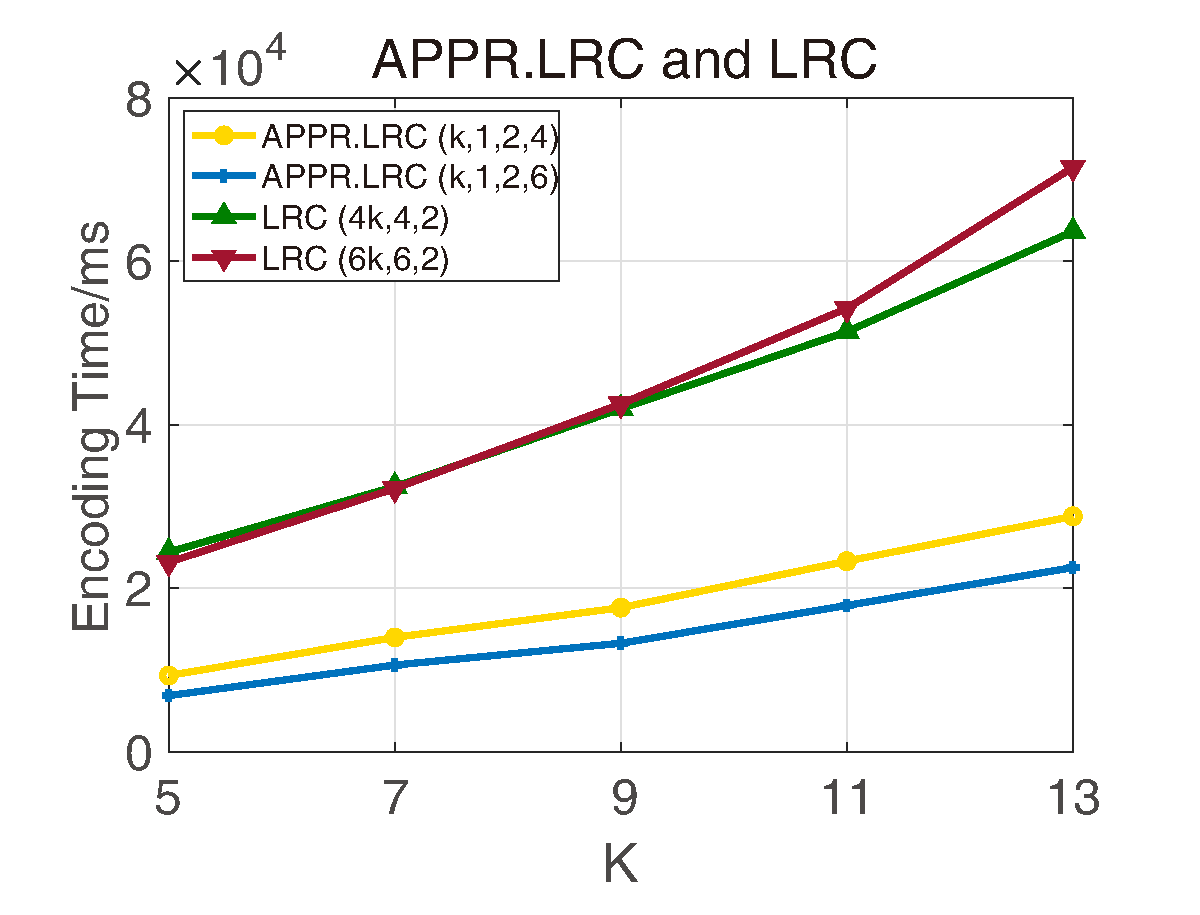
\includegraphics[width = 0.46\linewidth]{photo/experiment/Encoding-LRC.eps}
}

\caption{Encoding Time Comparison among various erasure coding methods.}\label{fig-encoding}

\end{figure}


\subsubsection{Decoding Time under Single Node Failure Condition}
The results are shown in Table \ref{tab-summary}.
\begin{itemize}
    \item Compared to STAR/TIP Codes: The decoding time of Approximate Code is almost the same as original code when single node fails, with an increment by up to $5.5\%$ for STAR code, up to $10.8\%$ for TIP-Code, respectively.
    \item Compared to RS/LRC Codes: Approximate Code decodes nearly the same as RS code (improvements by up to $0.9\%$) and LRC codes (enhancement by up to $1.3\%$).
    \item In some scenarios, Approximate Codes are worse than original codes, which is affected by small differences on parameter configurations.
\end{itemize}


\subsubsection{Decoding Time under Double Nodes Failure Condition}
The results are shown in Figure \ref{fig-decoding-2}.
\begin{itemize}
    \item Compared to STAR/TIP Codes: The recovery acceleration is up to $76.5\%$ for STAR, up to $77.6\%$, respectively.
    \item Compared to RS/LRC Codes: Approximate Code reconstruct the lost data faster than original erasure codes, which improve the reconstruction by up to $75.4\%$ for RS code, and $78.7\%$ for LRC codes, respectively.
\end{itemize}

\begin{figure}[ht]
\subfigure{
    \label{fig-decoding-2-STAR}
    \includegraphics[width = 0.46\linewidth]{photo/experiment/Decoding-2-Star.eps}
}
\subfigure{
    \label{fig-decoding-2-TIP}
    \includegraphics[width = 0.46\linewidth]{photo/experiment/Decoding-2-TIP.eps}
}
\subfigure{
    \label{fig-decoding-2-RS}
    \includegraphics[width = 0.46\linewidth]{photo/experiment/Decoding-2-RS.eps}
}
\subfigure{
    \label{fig-decoding-2-LRC}
    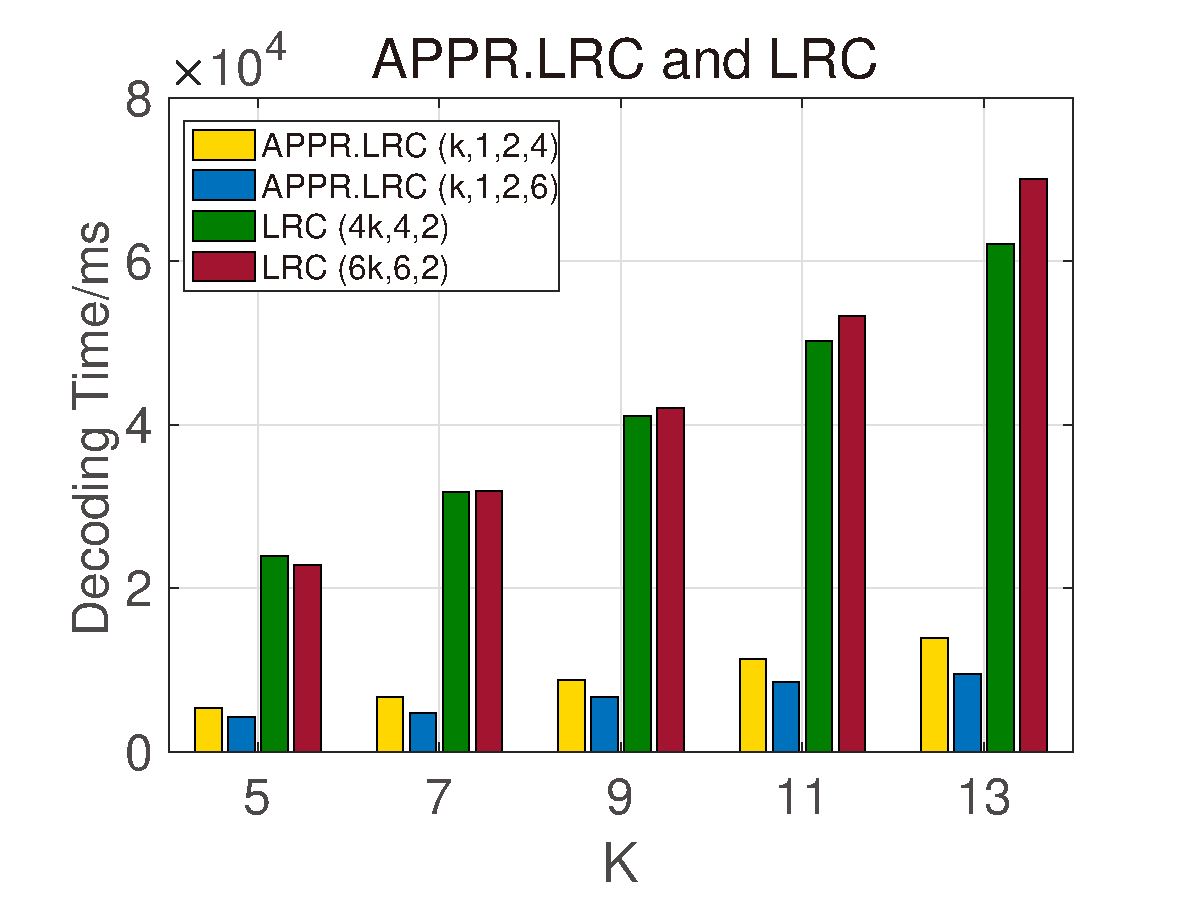
\includegraphics[width = 0.46\linewidth]{photo/experiment/Decoding-2-LRC.eps}
}

\caption{Double Nodes Decoding Time Comparison among various erasure coding methods.}\label{fig-decoding-2}
\end{figure}


\subsubsection{Decoding Time under Triple Nodes Failure Condition}
The results are shown in Figure \ref{fig-decoding-3}.
\begin{itemize}
    \item Compared to STAR Code: The maximum optimization ratio is $75.1\%$ (between APPR.STAR ($k,1,2,6$) and STAR ($k,3$) when $k = 5$).
    \item Compared to TIP-Code: This condition is similar to STAR code with an optimization ratio is up to $75.6\%$ (between APPR.TIP($k,1,2,6$) and TIP($k,3$) when $k = 9$).
    \item Compared to RS Code: Approximate Code decodes largely faster than RS code under three failure nodes condition by up to $75.0\%$ (between APPR.RS ($k,1,2,6$) and RS($k,3$) when $k = 5$).
    \item Compared to LRC Codes: Approximate Code largely reduces the decoding time  by up to $87.9\%$  (between APPR.LRC ($k,1,2,6$) and LRC ($k, 6, 2$) when $k = 13$).
\end{itemize}

We combined the encoding/decoding time of all erasure codes in Figure \ref{fig-BAR} when $k=5$. The results show that Approximate Code has the best encoding/decoding performance among all erasure codes. 

\begin{figure}[ht]
\subfigure{
    \label{fig-decoding-3-STAR}
    \includegraphics[width = 0.46\linewidth]{photo/experiment/Decoding-3-Star.eps}
}
\subfigure{
    \label{fig-decoding-3-TIP}
    \includegraphics[width = 0.46\linewidth]{photo/experiment/Decoding-3-TIP.eps}
}
\subfigure{
    \label{fig-decoding-3-RS}
    \includegraphics[width = 0.46\linewidth]{photo/experiment/Decoding-3-RS.eps}
}
\subfigure{
    \label{fig-decoding-3-LRC}
    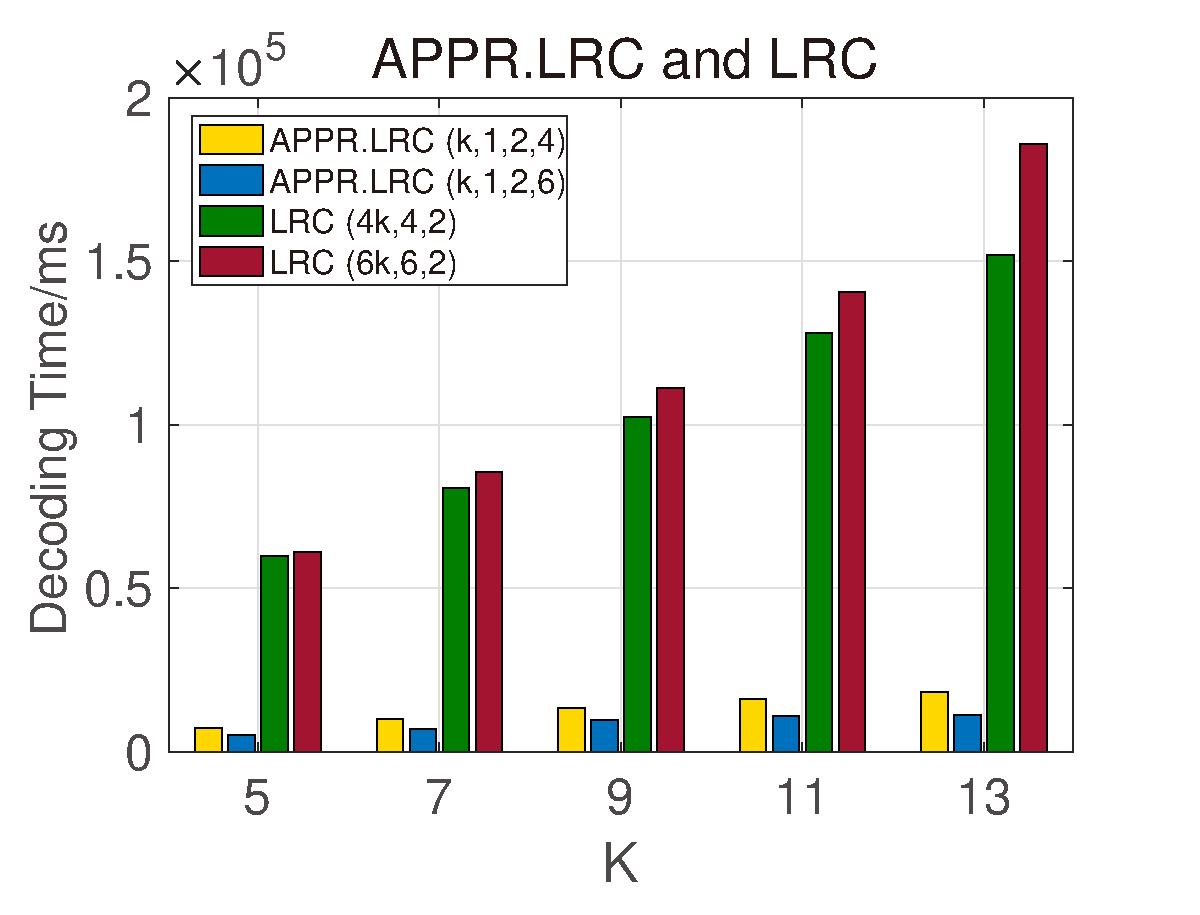
\includegraphics[width = 0.46\linewidth]{photo/experiment/Decoding-3-LRC.eps}
}

\caption{Triple Nodes Decoding Time Comparison among various erasure coding methods.}\label{fig-decoding-3}

\end{figure}

\begin{figure*}[ht]
\subfigure{
    \label{fig-encoding-combine}
    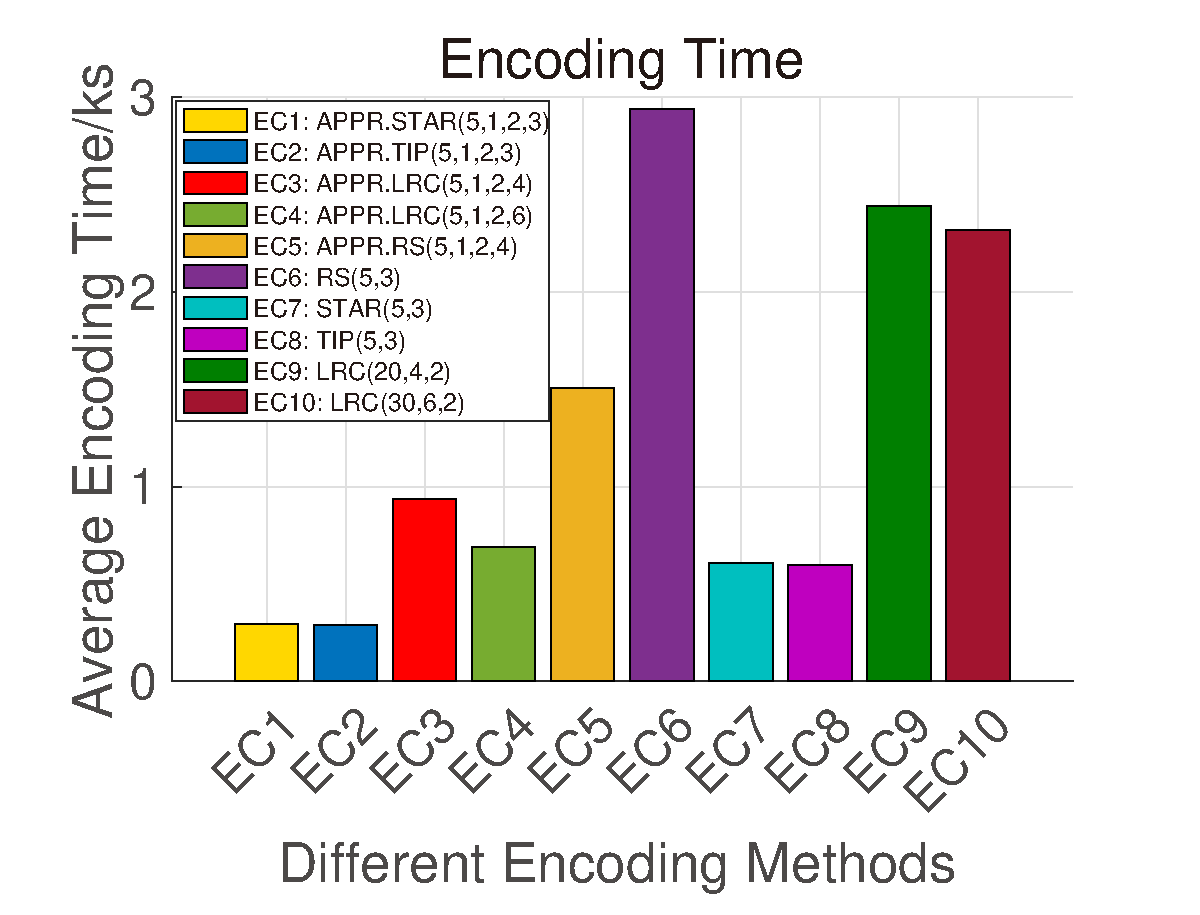
\includegraphics[width = 0.25\linewidth]{photo/experiment/Bar-Encoding.eps}
}\hspace{-3mm}
\subfigure{
    \label{fig-decoding-1-combine}
    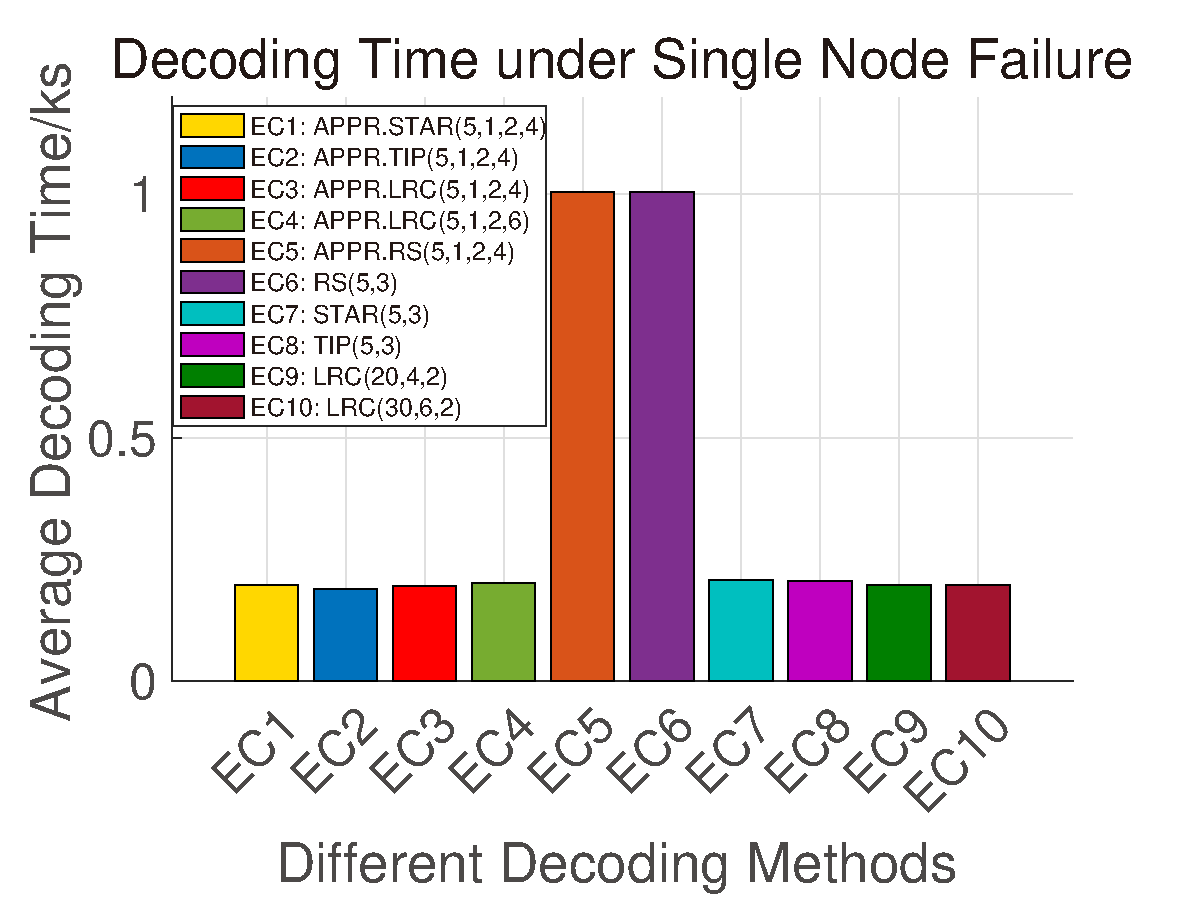
\includegraphics[width = 0.25\linewidth]{photo/experiment/Bar-Decoding-1.eps}
}\hspace{-3mm}
\subfigure{
    \label{fig-decoding-2-combine}
    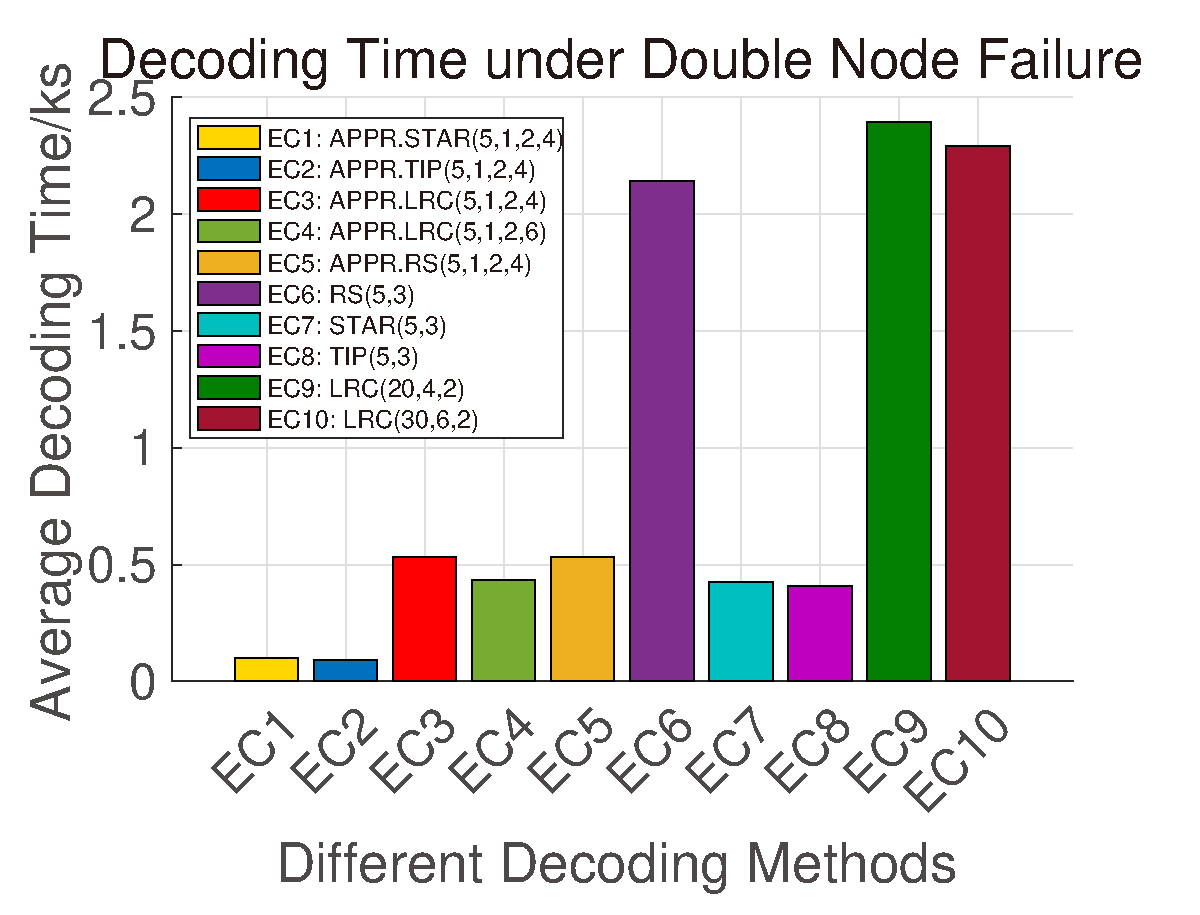
\includegraphics[width = 0.25\linewidth]{photo/experiment/Bar-Decoding-2.eps}
}\hspace{-3mm}
\subfigure{
    \label{fig-decoding-3-combine}
    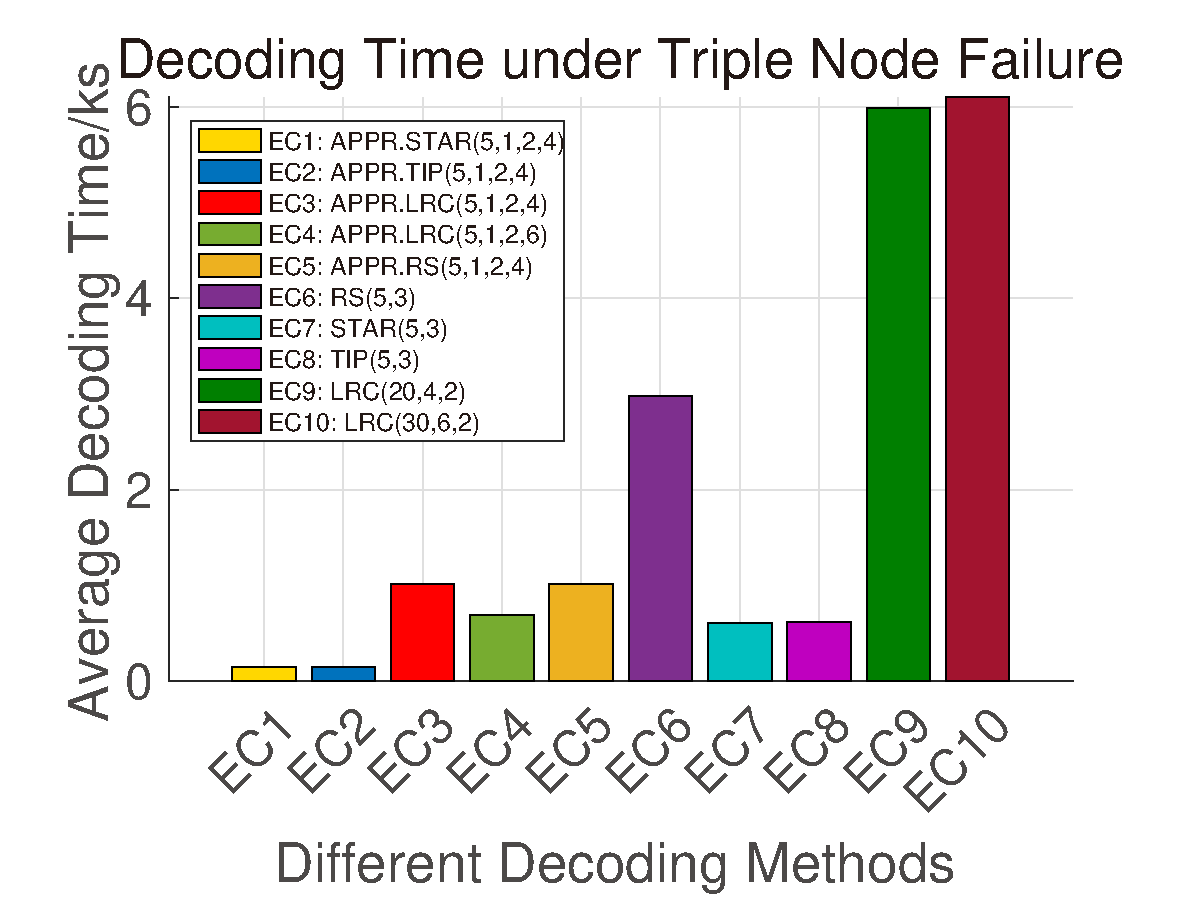
\includegraphics[width = 0.25\linewidth]{photo/experiment/Bar-Decoding-3.eps}
}

\caption{Comparison of several metrics with five data nodes ($k=5$).}\label{fig-BAR}

\end{figure*}

\subsubsection{Recovery Time}

Figure \ref{fig-recovery} shows the recovery time of various erasure codes (ECs) under two and three failure nodes
condition. We can see that Approximate Code owns the best recovery performance in all ECs. The optimization ratio is up to $95.9\%$.
The main reason is that Approximate Code only recover important data under multiple failure nodes condition which can significantly reduce computation time, I/O overhead and transmission time.


\begin{table}[]\footnotesize
\caption{Improvement of Approximate Codes ($k,1,2,4$) over their corresponding erasure codes.}\label{tab-summary}
\begin{tabular}{|c|c|c|c|c|c|c|}
\hline
Experiment & Coding & \multicolumn{5}{c|}{Number of Data Nodes} \\ \cline{3-7} 
Scenario & Method & 5 & 7 & 9 & 11 & 13 \\ \hline \hline
\multirow{4}{*}{Encoding} & RS & 48.80\% & 48.91\% & 53.96\% & 50.79\% & 51.90\% \\ \cline{2-7} 
 & STAR & 51.65\% & 51.04\% & / & 48.45\% & 46.92\% \\ \cline{2-7} 
 & TIP & 51.68\% & / & 54.29\% & 48.43\% & / \\ \cline{2-7} 
 & LRC & 61.69\% & 56.82\% & 57.95\% & 54.60\% & 54.71\% \\ \hline
Decoding & RS & 0.09\% & 0.89\% & 0.18\% & 0.62\% & 0.57\% \\ \cline{2-7} 
under & STAR & 5.50\% & 3.67\% & / & -2.05\% & -5.26\% \\ \cline{2-7} 
Single Node & TIP & 8.78\% & / & 10.79\% & -1.68\% & / \\ \cline{2-7} 
Failure & LRC & 1.32\% & -0.75\% & -0.91\% & -3.42\% & -9.54\% \\ \hline
Decoding & RS & 75.03\% & 75.35\% & 75.10\% & 75.23\% & 75.22\% \\ \cline{2-7} 
under & STAR & 76.46\% & 75.98\% & / & 74.54\% & 73.73\% \\ \cline{2-7} 
Double Node & TIP & 77.11\% & / & 77.63\% & 74.53\% & / \\ \cline{2-7} 
Failure & LRC & 77.75\% & 78.70\% & 78.53\% & 77.41\% & 77.62\% \\ \hline
Decoding & RS & 75.00\% & 75.01\% & 74.99\% & 74.99\% & 75.02\% \\ \cline{2-7} 
under & STAR & 75.11\% & 74.94\% & / & 75.11\% & 75.03\% \\ \cline{2-7} 
Triple Node & TIP & 74.85\% & / & 75.57\% & 73.23\% & / \\ \cline{2-7} 
Failure & LRC & 87.58\% & 87.40\% & 87.00\% & 87.29\% & 87.87\% \\ \hline
\end{tabular}
\end{table}


\begin{figure}[ht]
\subfigure[Double nodes recovery]{
    \label{fig-recovery-2}
    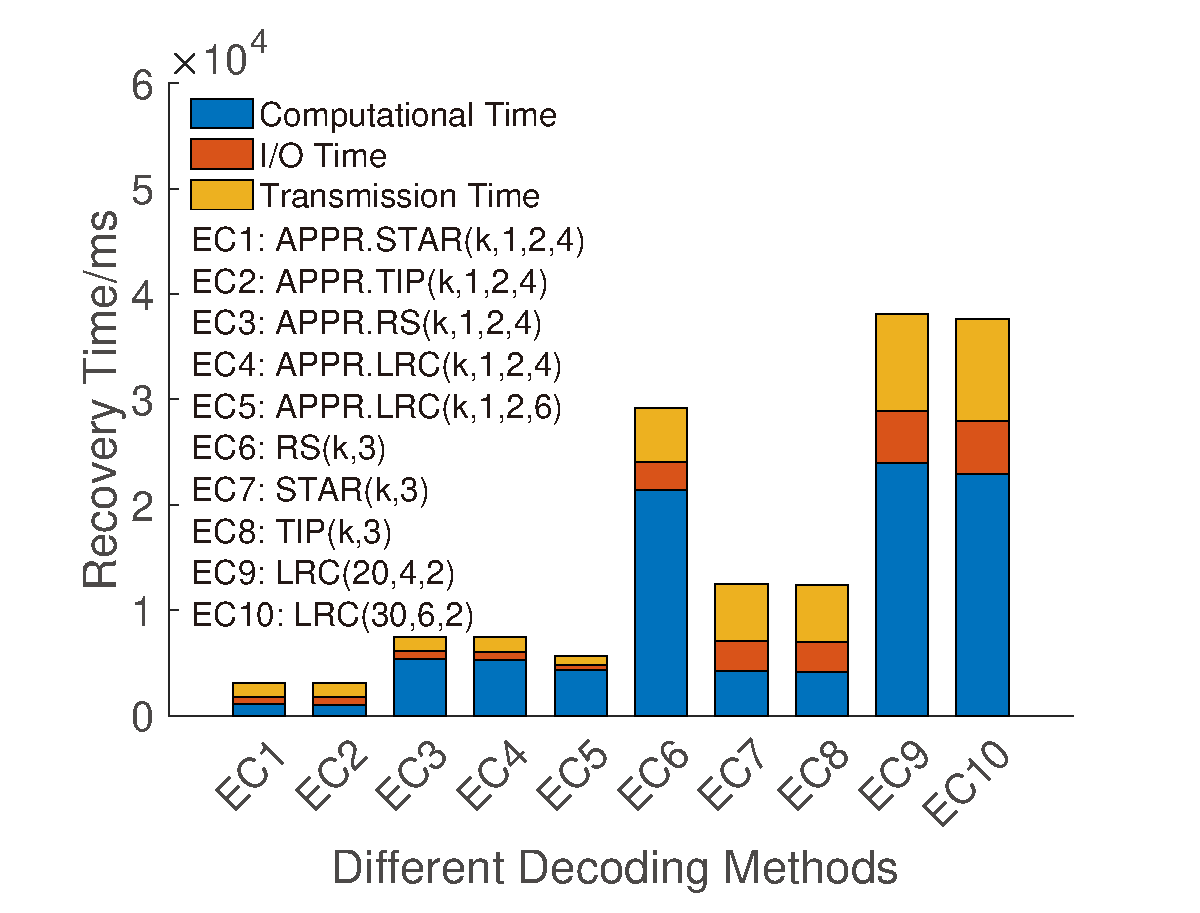
\includegraphics[width = 0.5\linewidth]{photo/experiment/Recovery-2.eps}
}\hspace{-4mm}
\subfigure[Triple nodes recovery]{
    \label{fig-recovery-3}
    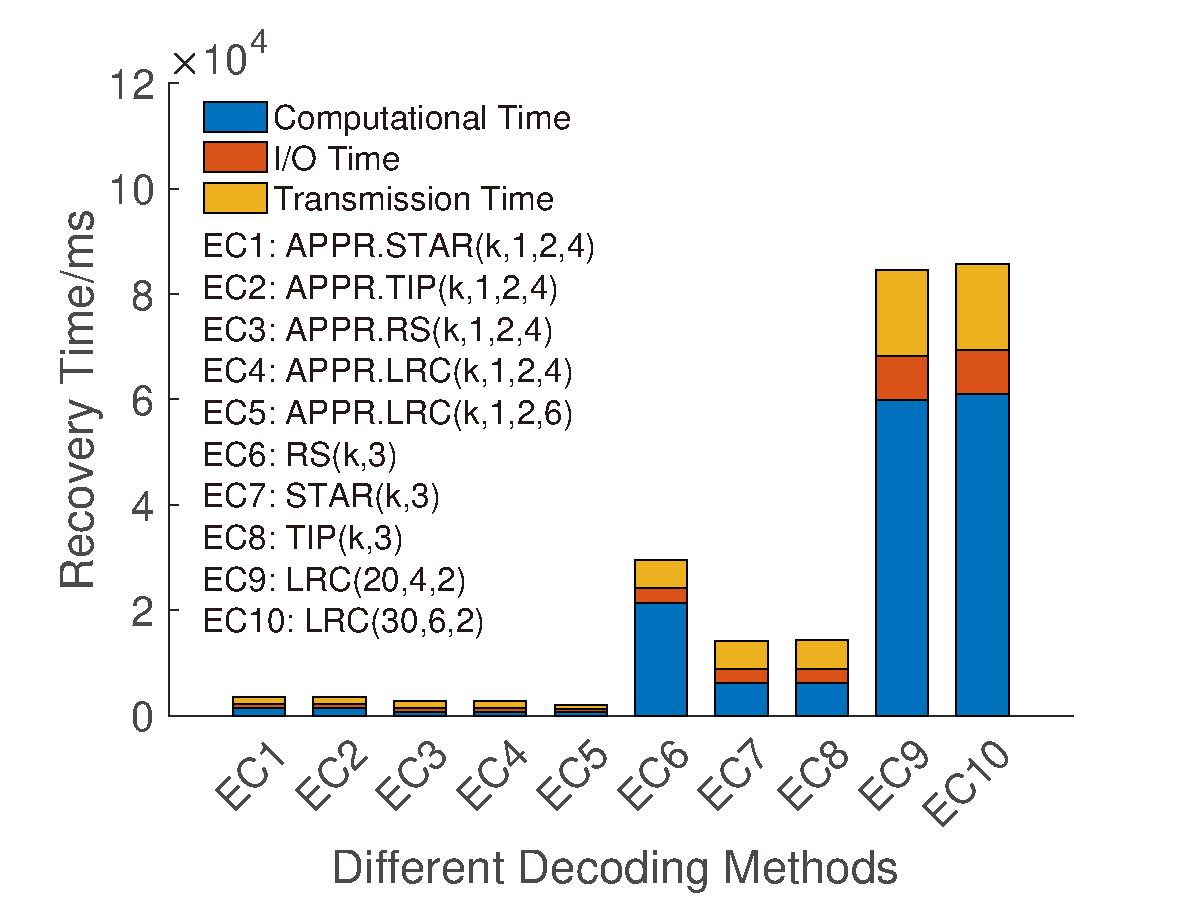
\includegraphics[width = 0.5\linewidth]{photo/experiment/Recovery-3.eps}
}

\caption{Recovery time comparison under double/triple nodes failure among various erasure coding methods.}\label{fig-recovery}

\end{figure}

\iffalse
\begin{figure}[ht]
\centering
\subfigure[Frame 1]{
\includegraphics[width=0.3\linewidth]{photo/Frame/1.jpg}\label{fig-interop1}
}
\subfigure[Frame 2]{
\includegraphics[width=0.3\linewidth]{photo/Frame/2.jpg}\label{fig-interop2}
}
\subfigure[Frame 3]{
\includegraphics[width=0.3\linewidth]{photo/Frame/3.jpg}\label{fig-interop3}
}

\subfigure[Recovery of Frame 2]{
\includegraphics[width=0.3\linewidth]{photo/Frame/2_1.jpg}\label{fig-recoverof2}
}
\caption{Video Recovery Result using Frame Interpolation.}
\label{fig-frameRecovery}
\end{figure}
\fi


\subsection{Analysis}
The improvements of Approximate Code over typical erasure codes are listed in Table \ref{tab-SO} and Table \ref{tab-summary}. From the table, we notice that Approximate Code is a cost-effective solution for 3DFTs. There are several reasons to achieve these gains. First, Approximate Code only provides triple parities for important data, which leads to the degradation of storage cost and improvements on encoding/decoding performance. Second, Approximate Code simplifies the generation of local parities, which reduces the computational complexity. Third, the parity chains in Approximate Code are short, which decreases the transmission time and I/O overhead in cloud storage systems.


\section{Conclusion}\label{Conclusion}
In this paper, we propose a novel erasure coding framework called Approximate Code, which is used for tiered video storage in cloud systems. The framework provides high reliability for important data and low reliability for unimportant. By this way, the storage cost can be saved. The experimental results show that Approximate Code have the following advantages, (1) reduces the number of parities by up to $55\%$, (2) saves the storage cost by up to $20.8\%$, (3) increases the recovery speed by up to a factor of $4.7X$ under double/triple nodes failure conditions.

\section*{Acknowledgement}
We thank anonymous reviewers for their insightful comments. This work is partially sponsored by the National Key R\&D Program of China (No.2018YFB0105203), the National 973 Program of China (No.2015CB352403), the Natural Science Foundation of Shanghai (No.18ZR1418500), the Alibaba Group through Alibaba Innovative Research (AIR) program, and the Open Research fund by Data Storage System Lab, Ministry of Education of China.

\bibliographystyle{ACM-Reference-Format}
\bibliography{ApproximateCode}

\end{document}
